\documentclass[twoside]{article}

% Packages required by doxygen
\usepackage{fixltx2e}
\usepackage{calc}
\usepackage{doxygen}
\usepackage[export]{adjustbox} % also loads graphicx
\usepackage{graphicx}
\usepackage[utf8]{inputenc}
\usepackage{makeidx}
\usepackage{multicol}
\usepackage{multirow}
\PassOptionsToPackage{warn}{textcomp}
\usepackage{textcomp}
\usepackage[nointegrals]{wasysym}
\usepackage[table]{xcolor}

% Font selection
\usepackage[T1]{fontenc}
\usepackage[scaled=.90]{helvet}
\usepackage{courier}
\usepackage{amssymb}
\usepackage{sectsty}
\renewcommand{\familydefault}{\sfdefault}
\allsectionsfont{%
  \fontseries{bc}\selectfont%
  \color{darkgray}%
}
\renewcommand{\DoxyLabelFont}{%
  \fontseries{bc}\selectfont%
  \color{darkgray}%
}
\newcommand{\+}{\discretionary{\mbox{\scriptsize$\hookleftarrow$}}{}{}}

% Page & text layout
\usepackage{geometry}
\geometry{%
  a4paper,%
  top=2.5cm,%
  bottom=2.5cm,%
  left=2.5cm,%
  right=2.5cm%
}
\tolerance=750
\hfuzz=15pt
\hbadness=750
\setlength{\emergencystretch}{15pt}
\setlength{\parindent}{0cm}
\setlength{\parskip}{3ex plus 2ex minus 2ex}
\makeatletter
\renewcommand{\paragraph}{%
  \@startsection{paragraph}{4}{0ex}{-1.0ex}{1.0ex}{%
    \normalfont\normalsize\bfseries\SS@parafont%
  }%
}
\renewcommand{\subparagraph}{%
  \@startsection{subparagraph}{5}{0ex}{-1.0ex}{1.0ex}{%
    \normalfont\normalsize\bfseries\SS@subparafont%
  }%
}
\makeatother

% Headers & footers
\usepackage{fancyhdr}
\pagestyle{fancyplain}
\fancyhead[LE]{\fancyplain{}{\bfseries\thepage}}
\fancyhead[CE]{\fancyplain{}{}}
\fancyhead[RE]{\fancyplain{}{\bfseries\leftmark}}
\fancyhead[LO]{\fancyplain{}{\bfseries\rightmark}}
\fancyhead[CO]{\fancyplain{}{}}
\fancyhead[RO]{\fancyplain{}{\bfseries\thepage}}
\fancyfoot[LE]{\fancyplain{}{}}
\fancyfoot[CE]{\fancyplain{}{}}
\fancyfoot[RE]{\fancyplain{}{\bfseries\scriptsize Generated by Doxygen }}
\fancyfoot[LO]{\fancyplain{}{\bfseries\scriptsize Generated by Doxygen }}
\fancyfoot[CO]{\fancyplain{}{}}
\fancyfoot[RO]{\fancyplain{}{}}
\renewcommand{\footrulewidth}{0.4pt}
\renewcommand{\sectionmark}[1]{%
  \markright{\thesection\ #1}%
}

% Indices & bibliography
\usepackage{natbib}
\usepackage[titles]{tocloft}
\setcounter{tocdepth}{3}
\setcounter{secnumdepth}{5}
\makeindex

% Hyperlinks (required, but should be loaded last)
\usepackage{ifpdf}
\ifpdf
  \usepackage[pdftex,pagebackref=true]{hyperref}
\else
  \usepackage[ps2pdf,pagebackref=true]{hyperref}
\fi
\hypersetup{%
  colorlinks=true,%
  linkcolor=blue,%
  citecolor=blue,%
  unicode%
}

% Custom commands
\newcommand{\clearemptydoublepage}{%
  \newpage{\pagestyle{empty}\cleardoublepage}%
}

\usepackage{caption}
\captionsetup{labelsep=space,justification=centering,font={bf},singlelinecheck=off,skip=4pt,position=top}

%===== C O N T E N T S =====

\begin{document}

% Titlepage & ToC
\hypersetup{pageanchor=false,
             bookmarksnumbered=true,
             pdfencoding=unicode
            }
\pagenumbering{roman}
\begin{titlepage}
\vspace*{7cm}
\begin{center}%
{\Large General U\+ML Statemachine Implementation \\[1ex]\large 0000 }\\
\vspace*{1cm}
{\large Generated by Doxygen 1.8.11}\\
\end{center}
\end{titlepage}
\tableofcontents
\pagenumbering{arabic}
\hypersetup{pageanchor=true}

%--- Begin generated contents ---
\section{Main Page}
\label{index}\hypertarget{index}{}\subsubsection*{U\+ML state machines (main source wikipedia)}

The Unified Modeling Language has a notation for describing state machines. U\+ML state machines overcome the limitations of traditional finite state machines while retaining their main benefits.

 
\begin{DoxyImage}
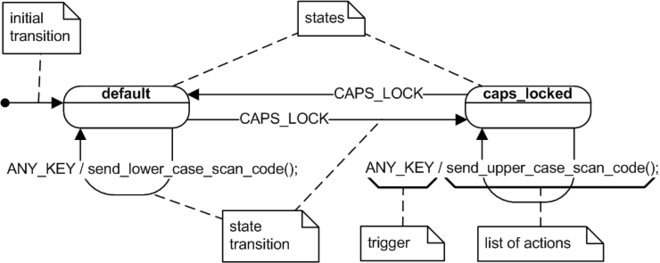
\includegraphics[width=10cm]{basic_uml_state_chart.png}
\caption{Basic U\+ML state chart}
\end{DoxyImage}


U\+ML state machines introduce the new concepts of hierarchically nested states and orthogonal regions, while extending the notion of actions. U\+ML state machines have the characteristics of both Mealy machines and Moore machines. They support actions that depend on both the state of the system and the triggering event, as in Mealy machines, as well as entry and exit actions, which are associated with states rather than transitions, as in Moore machines.

\subsubsection*{Supported features in this implementation (main source wikipedia)}

\paragraph*{Events}

An event is something that happens that affects the system. Strictly speaking, in the U\+ML specification, the term event refers to the type of occurrence rather than to any concrete instance of that occurrence.

An event can have associated parameters, allowing the event instance to convey not only the occurrence of some interesting incident but also quantitative information regarding that occurrence.

An event instance outlives the instantaneous occurrence that generated it and might convey this occurrence to one or more state machines. Once generated, the event instance goes through a processing life cycle that can consist of up to three stages. First, the event instance is received when it is accepted and waiting for processing (e.\+g., it is placed on the event queue). Later, the event instance is dispatched to the state machine, at which point it becomes the current event. Finally, it is consumed when the state machine finishes processing the event instance. A consumed event instance is no longer available for processing.

\paragraph*{States}

A state captures the relevant aspects of the system\textquotesingle{}s history very efficiently. To relate this concept to programming, this means that instead of recording the event history in a multitude of variables, flags, and convoluted logic, you rely mainly on just one state variable that can assume only a limited number of a priori determined values. The value of the state variable crisply defines the current state of the system at any given time. The concept of state reduces the problem of identifying the execution context in the code to testing just the state variable instead of many variables, thus eliminating a lot of conditional logic. Moreover, switching between different states

\paragraph*{Guard conditions}

Guard conditions (or simply guards) are Boolean expressions evaluated dynamically based on the value of extended state variables and event parameters. Guard conditions affect the behavior of a state machine by enabling actions or transitions only when they evaluate to T\+R\+UE and disabling them when they evaluate to F\+A\+L\+SE. In the U\+ML notation, guard conditions are shown in square brackets.

The need for guards is the immediate consequence of adding memory extended state variables to the state machine formalism. Used sparingly, extended state variables and guards make up a powerful mechanism that can simplify designs. But don not let the fancy name (\char`\"{}guard\char`\"{}) and the concise U\+ML notation fool you. When you actually code an extended state machine, the guards become the same I\+Fs and E\+L\+S\+Es that you wanted to eliminate by using the state machine in the first place. Too many of them, and you will find yourself back in square one (\char`\"{}spaghetti code\char`\"{}), where the guards effectively take over handling of all the relevant conditions in the system.

\paragraph*{Actions and transitions}

When an event instance is dispatched, the state machine responds by performing actions, such as changing a variable, performing I/O, invoking a function, generating another event instance, or changing to another state. Any parameter values associated with the current event are available to all actions directly caused by that event. Switching from one state to another is called state transition, and the event that causes it is called the triggering event, or simply the trigger.

\paragraph*{Entry and exit actions}

Every state in a U\+ML statechart can have optional entry actions, which are executed upon entry to a state, as well as optional exit actions, which are executed upon exit from a state. Entry and exit actions are associated with states, not transitions.

 
\begin{DoxyImage}
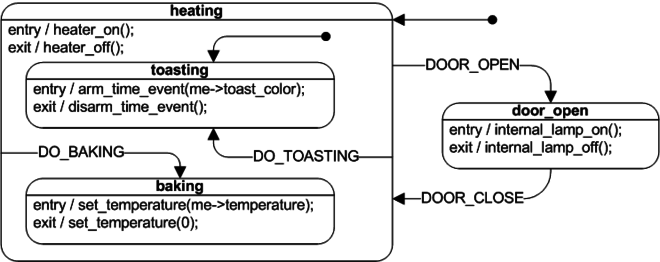
\includegraphics[width=10cm]{entry_exit_actions.png}
\caption{Entry/\+Exit Actions}
\end{DoxyImage}


Regardless of how a state is entered or exited, all its entry and exit actions will be executed. Because of this characteristic, statecharts behave like Moore machines. The U\+ML notation for state entry and exit actions is to place the reserved word \char`\"{}entry\char`\"{} (or \char`\"{}exit\char`\"{}) in the state right below the name compartment, followed by the forward slash and the list of arbitrary actions.

\paragraph*{Internal transitions}

Very commonly, an event causes only some internal actions to execute but does not lead to a change of state (state transition). In this case, all actions executed comprise the internal transition. In the absence of entry and exit actions, internal transitions would be identical to self-\/transitions (transitions in which the target state is the same as the source state).

 
\begin{DoxyImage}
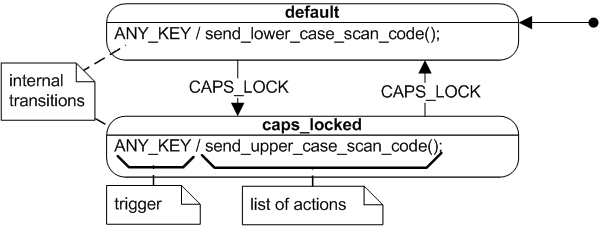
\includegraphics[width=10cm]{internal_transition.png}
\caption{Internal Transitions}
\end{DoxyImage}


In fact, in a classical Mealy machine, actions are associated exclusively with state transitions, so the only way to execute actions without changing state is through a self-\/transition. However, in the presence of entry and exit actions, as in U\+ML statecharts, a self-\/transition involves the execution of exit and entry actions and therefore it is distinctively different from an internal transition. 
\section{Module Index}
\subsection{Modules}
Here is a list of all modules\+:\begin{DoxyCompactList}
\item \contentsline{section}{Public Interface Descriptions}{\pageref{group___public_interfaces}}{}
\begin{DoxyCompactList}
\item \contentsline{section}{Public Statemachine Interface}{\pageref{group___sm_interface}}{}
\end{DoxyCompactList}
\end{DoxyCompactList}

\section{Data Structure Index}
\subsection{Data Structures}
Here are the data structures with brief descriptions\+:\begin{DoxyCompactList}
\item\contentsline{section}{\hyperlink{structsm__state__t}{sm\+\_\+state\+\_\+t} }{\pageref{structsm__state__t}}{}
\item\contentsline{section}{\hyperlink{structsm__t}{sm\+\_\+t} \\*Statemachine declaration }{\pageref{structsm__t}}{}
\end{DoxyCompactList}

\section{File Index}
\subsection{File List}
Here is a list of all files with brief descriptions\+:\begin{DoxyCompactList}
\item\contentsline{section}{src/\hyperlink{main_8c}{main.\+c} \\*Main entry point of application }{\pageref{main_8c}}{}
\item\contentsline{section}{src/\hyperlink{sm_8c}{sm.\+c} \\*General U\+ML state machine implementation }{\pageref{sm_8c}}{}
\item\contentsline{section}{src/\hyperlink{sm_8h}{sm.\+h} \\*General U\+ML state machine interface }{\pageref{sm_8h}}{}
\item\contentsline{section}{src/\hyperlink{statemachine_8c}{statemachine.\+c} \\*Statemachine for testing purposes -\/ implementation }{\pageref{statemachine_8c}}{}
\item\contentsline{section}{src/\hyperlink{statemachine_8h}{statemachine.\+h} \\*Statemachine for testing purposes -\/ interface }{\pageref{statemachine_8h}}{}
\end{DoxyCompactList}

\section{Module Documentation}
\hypertarget{group___public_interfaces}{}\subsection{Public Interface Descriptions}
\label{group___public_interfaces}\index{Public Interface Descriptions@{Public Interface Descriptions}}
Collaboration diagram for Public Interface Descriptions\+:\nopagebreak
\begin{figure}[H]
\begin{center}
\leavevmode
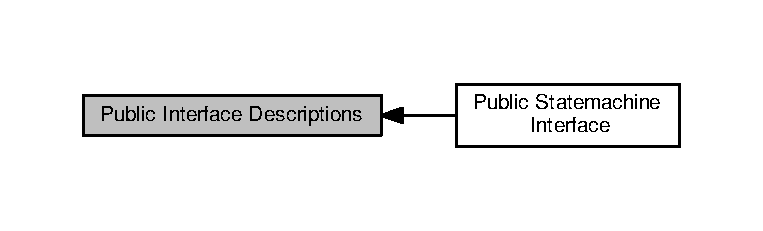
\includegraphics[width=350pt]{group___public_interfaces}
\end{center}
\end{figure}
\subsubsection*{Modules}
\begin{DoxyCompactItemize}
\item 
\hyperlink{group___sm_interface}{Public Statemachine Interface}
\end{DoxyCompactItemize}


\subsubsection{Detailed Description}

\hypertarget{group___sm_interface}{}\subsection{Public Statemachine Interface}
\label{group___sm_interface}\index{Public Statemachine Interface@{Public Statemachine Interface}}
Collaboration diagram for Public Statemachine Interface\+:\nopagebreak
\begin{figure}[H]
\begin{center}
\leavevmode
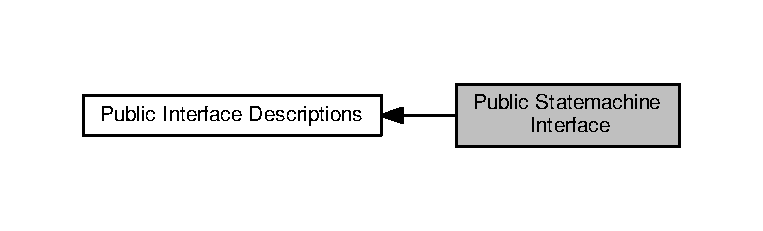
\includegraphics[width=350pt]{group___sm_interface}
\end{center}
\end{figure}
\subsubsection*{Functions}
\begin{DoxyCompactItemize}
\item 
\hyperlink{structsm__state__t}{sm\+\_\+state\+\_\+t} $\ast$ \hyperlink{group___sm_interface_ga4d433df4f0fbd1033d3815ad870cdc5f}{sm\+\_\+init} (\hyperlink{structsm__t}{sm\+\_\+t} $\ast$sm, const \hyperlink{structsm__state__t}{sm\+\_\+state\+\_\+t} $\ast$state)
\begin{DoxyCompactList}\small\item\em Initialize a statemachine with a provided initial state. \end{DoxyCompactList}\item 
void \hyperlink{group___sm_interface_ga4a0ade9dfadc3d8a476cd64934ee369c}{sm\+\_\+terminate} (\hyperlink{structsm__t}{sm\+\_\+t} $\ast$sm)
\begin{DoxyCompactList}\small\item\em Terminates the statemachine. \end{DoxyCompactList}\item 
\hyperlink{structsm__state__t}{sm\+\_\+state\+\_\+t} $\ast$ \hyperlink{group___sm_interface_gac4c2466939ae8d63448dc84848abb7fe}{sm\+\_\+send} (\hyperlink{structsm__t}{sm\+\_\+t} $\ast$sm, \hyperlink{sm_8h_a1db78734760bf970c329945446b28432}{event\+\_\+t} event, void $\ast$data)
\begin{DoxyCompactList}\small\item\em Sends an event to a statemachine. \end{DoxyCompactList}\end{DoxyCompactItemize}


\subsubsection{Detailed Description}


\subsubsection{Function Documentation}
\index{Public Statemachine Interface@{Public Statemachine Interface}!sm\+\_\+init@{sm\+\_\+init}}
\index{sm\+\_\+init@{sm\+\_\+init}!Public Statemachine Interface@{Public Statemachine Interface}}
\paragraph[{\texorpdfstring{sm\+\_\+init(sm\+\_\+t $\ast$sm, const sm\+\_\+state\+\_\+t $\ast$state)}{sm_init(sm_t *sm, const sm_state_t *state)}}]{\setlength{\rightskip}{0pt plus 5cm}{\bf sm\+\_\+state\+\_\+t}$\ast$ sm\+\_\+init (
\begin{DoxyParamCaption}
\item[{{\bf sm\+\_\+t} $\ast$}]{sm, }
\item[{const {\bf sm\+\_\+state\+\_\+t} $\ast$}]{state}
\end{DoxyParamCaption}
)}\hypertarget{group___sm_interface_ga4d433df4f0fbd1033d3815ad870cdc5f}{}\label{group___sm_interface_ga4d433df4f0fbd1033d3815ad870cdc5f}


Initialize a statemachine with a provided initial state. 

Initializes the statemachine with a provided state. The Initial State from the U\+ML Statechart Diagram is the state of an object before any transitions. The Initial State from the U\+ML Statechart Diagram marks the entry point and the initial statemachine state. The notation for the Initial State is a small solid filled circle. There can only be one Initial State on a diagram. Invoking this function transits from initial pseudo state to the initial statemachine state.


\begin{DoxyParams}[1]{Parameters}
\mbox{\tt in,out}  & {\em sm} & State machine instance \\
\hline
\mbox{\tt in}  & {\em state} & State to initialize the state machine with. Has to be a valid state of the state machines state table.\\
\hline
\end{DoxyParams}
\begin{DoxyReturn}{Returns}
State of the state machine after initial transition. N\+U\+LL if initialization failed 
\end{DoxyReturn}


Definition at line 116 of file sm.\+c.



Here is the caller graph for this function\+:\nopagebreak
\begin{figure}[H]
\begin{center}
\leavevmode
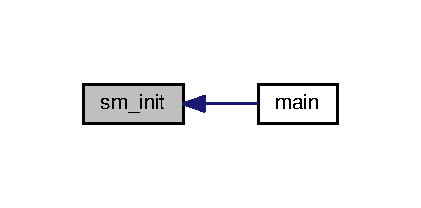
\includegraphics[width=202pt]{group___sm_interface_ga4d433df4f0fbd1033d3815ad870cdc5f_icgraph}
\end{center}
\end{figure}


\index{Public Statemachine Interface@{Public Statemachine Interface}!sm\+\_\+send@{sm\+\_\+send}}
\index{sm\+\_\+send@{sm\+\_\+send}!Public Statemachine Interface@{Public Statemachine Interface}}
\paragraph[{\texorpdfstring{sm\+\_\+send(sm\+\_\+t $\ast$sm, event\+\_\+t event, void $\ast$data)}{sm_send(sm_t *sm, event_t event, void *data)}}]{\setlength{\rightskip}{0pt plus 5cm}{\bf sm\+\_\+state\+\_\+t}$\ast$ sm\+\_\+send (
\begin{DoxyParamCaption}
\item[{{\bf sm\+\_\+t} $\ast$}]{sm, }
\item[{{\bf event\+\_\+t}}]{event, }
\item[{void $\ast$}]{data}
\end{DoxyParamCaption}
)}\hypertarget{group___sm_interface_gac4c2466939ae8d63448dc84848abb7fe}{}\label{group___sm_interface_gac4c2466939ae8d63448dc84848abb7fe}


Sends an event to a statemachine. 


\begin{DoxyParams}[1]{Parameters}
\mbox{\tt in,out}  & {\em sm} & State machine instance \\
\hline
\mbox{\tt in}  & {\em event} & Event to be sent to the state machine \\
\hline
\mbox{\tt in,out}  & {\em data} & Data associated with the event\\
\hline
\end{DoxyParams}
\begin{DoxyReturn}{Returns}
State of the state machine after transition. N\+U\+LL if transition failed. 
\end{DoxyReturn}


Definition at line 166 of file sm.\+c.



Here is the caller graph for this function\+:\nopagebreak
\begin{figure}[H]
\begin{center}
\leavevmode
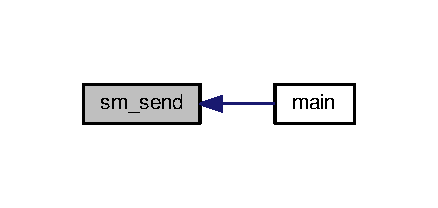
\includegraphics[width=210pt]{group___sm_interface_gac4c2466939ae8d63448dc84848abb7fe_icgraph}
\end{center}
\end{figure}


\index{Public Statemachine Interface@{Public Statemachine Interface}!sm\+\_\+terminate@{sm\+\_\+terminate}}
\index{sm\+\_\+terminate@{sm\+\_\+terminate}!Public Statemachine Interface@{Public Statemachine Interface}}
\paragraph[{\texorpdfstring{sm\+\_\+terminate(sm\+\_\+t $\ast$sm)}{sm_terminate(sm_t *sm)}}]{\setlength{\rightskip}{0pt plus 5cm}void sm\+\_\+terminate (
\begin{DoxyParamCaption}
\item[{{\bf sm\+\_\+t} $\ast$}]{sm}
\end{DoxyParamCaption}
)}\hypertarget{group___sm_interface_ga4a0ade9dfadc3d8a476cd64934ee369c}{}\label{group___sm_interface_ga4a0ade9dfadc3d8a476cd64934ee369c}


Terminates the statemachine. 

This function is meant to be used to terminate a statemachine. Usually a statemachine terminates itself by entering a pseudo final state.


\begin{DoxyParams}[1]{Parameters}
\mbox{\tt in,out}  & {\em sm} & State machine instance \\
\hline
\end{DoxyParams}


Definition at line 140 of file sm.\+c.


\section{Data Structure Documentation}
\hypertarget{structsm__state__t}{}\subsection{sm\+\_\+state\+\_\+t Struct Reference}
\label{structsm__state__t}\index{sm\+\_\+state\+\_\+t@{sm\+\_\+state\+\_\+t}}


{\ttfamily \#include $<$sm.\+h$>$}



Collaboration diagram for sm\+\_\+state\+\_\+t\+:\nopagebreak
\begin{figure}[H]
\begin{center}
\leavevmode
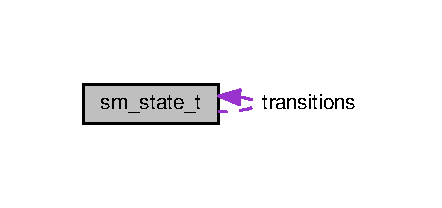
\includegraphics[width=212pt]{structsm__state__t__coll__graph}
\end{center}
\end{figure}
\subsubsection*{Data Fields}
\begin{DoxyCompactItemize}
\item 
\hyperlink{sm_8h_a921fca7daf06810fad2eca72b5a0bafc}{sm\+\_\+entry\+\_\+action\+\_\+fp} \hyperlink{structsm__state__t_ae5671e79c3bc83130bdeaf82c82e6f05}{entry\+\_\+action}
\item 
\hyperlink{sm_8h_a48bd707c3bca2429aee6582bd67cd273}{sm\+\_\+transitions\+\_\+fp} \hyperlink{structsm__state__t_ace0f4ad76339cbc43c48c99df054e401}{transitions}
\item 
\hyperlink{sm_8h_a0b45d5fb53866f3e67285aa38b248570}{sm\+\_\+exit\+\_\+action\+\_\+fp} \hyperlink{structsm__state__t_af372299be3ffdd7c40f91d0c0239839a}{exit\+\_\+action}
\end{DoxyCompactItemize}


\subsubsection{Detailed Description}
A state captures the relevant aspects of the system\textquotesingle{}s history very efficiently. The state of an object is always determined by its attributes and associations. States in state chart diagrams represent a set of those value combinations, in which an object behaves the same in response to events. 

Definition at line 165 of file sm.\+h.



\subsubsection{Field Documentation}
\index{sm\+\_\+state\+\_\+t@{sm\+\_\+state\+\_\+t}!entry\+\_\+action@{entry\+\_\+action}}
\index{entry\+\_\+action@{entry\+\_\+action}!sm\+\_\+state\+\_\+t@{sm\+\_\+state\+\_\+t}}
\paragraph[{\texorpdfstring{entry\+\_\+action}{entry_action}}]{\setlength{\rightskip}{0pt plus 5cm}{\bf sm\+\_\+entry\+\_\+action\+\_\+fp} entry\+\_\+action}\hypertarget{structsm__state__t_ae5671e79c3bc83130bdeaf82c82e6f05}{}\label{structsm__state__t_ae5671e79c3bc83130bdeaf82c82e6f05}
entry action to be performed if the state gets entered 

Definition at line 166 of file sm.\+h.

\index{sm\+\_\+state\+\_\+t@{sm\+\_\+state\+\_\+t}!exit\+\_\+action@{exit\+\_\+action}}
\index{exit\+\_\+action@{exit\+\_\+action}!sm\+\_\+state\+\_\+t@{sm\+\_\+state\+\_\+t}}
\paragraph[{\texorpdfstring{exit\+\_\+action}{exit_action}}]{\setlength{\rightskip}{0pt plus 5cm}{\bf sm\+\_\+exit\+\_\+action\+\_\+fp} exit\+\_\+action}\hypertarget{structsm__state__t_af372299be3ffdd7c40f91d0c0239839a}{}\label{structsm__state__t_af372299be3ffdd7c40f91d0c0239839a}
exit action to be performed if the state gets exited 

Definition at line 168 of file sm.\+h.

\index{sm\+\_\+state\+\_\+t@{sm\+\_\+state\+\_\+t}!transitions@{transitions}}
\index{transitions@{transitions}!sm\+\_\+state\+\_\+t@{sm\+\_\+state\+\_\+t}}
\paragraph[{\texorpdfstring{transitions}{transitions}}]{\setlength{\rightskip}{0pt plus 5cm}{\bf sm\+\_\+transitions\+\_\+fp} transitions}\hypertarget{structsm__state__t_ace0f4ad76339cbc43c48c99df054e401}{}\label{structsm__state__t_ace0f4ad76339cbc43c48c99df054e401}
external,internal and self transitions of the state 

Definition at line 167 of file sm.\+h.



The documentation for this struct was generated from the following file\+:\begin{DoxyCompactItemize}
\item 
src/\hyperlink{sm_8h}{sm.\+h}\end{DoxyCompactItemize}

\hypertarget{structsm__t}{}\subsection{sm\+\_\+t Struct Reference}
\label{structsm__t}\index{sm\+\_\+t@{sm\+\_\+t}}


Statemachine declaration.  




{\ttfamily \#include $<$sm.\+h$>$}



Collaboration diagram for sm\+\_\+t\+:\nopagebreak
\begin{figure}[H]
\begin{center}
\leavevmode
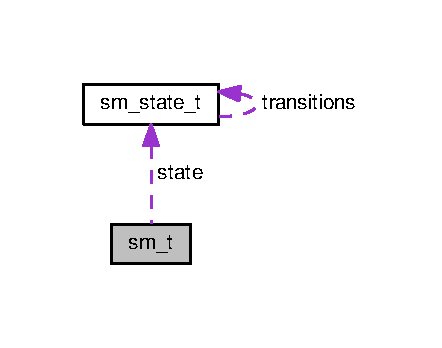
\includegraphics[width=212pt]{structsm__t__coll__graph}
\end{center}
\end{figure}
\subsubsection*{Data Fields}
\begin{DoxyCompactItemize}
\item 
\hyperlink{structsm__state__t}{sm\+\_\+state\+\_\+t} $\ast$ \hyperlink{structsm__t_ab950ad4739c4f74fc7070daba557c707}{state}
\item 
void $\ast$ \hyperlink{structsm__t_a735984d41155bc1032e09bece8f8d66d}{data}
\end{DoxyCompactItemize}


\subsubsection{Detailed Description}
Statemachine declaration. 

Holds the current state and data associated with the statemachine. 

Definition at line 175 of file sm.\+h.



\subsubsection{Field Documentation}
\index{sm\+\_\+t@{sm\+\_\+t}!data@{data}}
\index{data@{data}!sm\+\_\+t@{sm\+\_\+t}}
\paragraph[{\texorpdfstring{data}{data}}]{\setlength{\rightskip}{0pt plus 5cm}void$\ast$ data}\hypertarget{structsm__t_a735984d41155bc1032e09bece8f8d66d}{}\label{structsm__t_a735984d41155bc1032e09bece8f8d66d}
(Object-\/) Data associated with the statemachine 

Definition at line 177 of file sm.\+h.

\index{sm\+\_\+t@{sm\+\_\+t}!state@{state}}
\index{state@{state}!sm\+\_\+t@{sm\+\_\+t}}
\paragraph[{\texorpdfstring{state}{state}}]{\setlength{\rightskip}{0pt plus 5cm}{\bf sm\+\_\+state\+\_\+t}$\ast$ state}\hypertarget{structsm__t_ab950ad4739c4f74fc7070daba557c707}{}\label{structsm__t_ab950ad4739c4f74fc7070daba557c707}
Current state of the statemachine 

Definition at line 176 of file sm.\+h.



The documentation for this struct was generated from the following file\+:\begin{DoxyCompactItemize}
\item 
src/\hyperlink{sm_8h}{sm.\+h}\end{DoxyCompactItemize}

\section{File Documentation}
\hypertarget{mainpage_8dox}{}\subsection{doxy/mainpage.dox File Reference}
\label{mainpage_8dox}\index{doxy/mainpage.\+dox@{doxy/mainpage.\+dox}}

\hypertarget{modules_8dox}{}\subsection{doxy/modules.dox File Reference}
\label{modules_8dox}\index{doxy/modules.\+dox@{doxy/modules.\+dox}}

\hypertarget{main_8c}{}\subsection{src/main.c File Reference}
\label{main_8c}\index{src/main.\+c@{src/main.\+c}}


Main entry point of application.  


{\ttfamily \#include $<$stdio.\+h$>$}\\*
{\ttfamily \#include $<$stdlib.\+h$>$}\\*
{\ttfamily \#include \char`\"{}statemachine.\+h\char`\"{}}\\*
Include dependency graph for main.\+c\+:\nopagebreak
\begin{figure}[H]
\begin{center}
\leavevmode
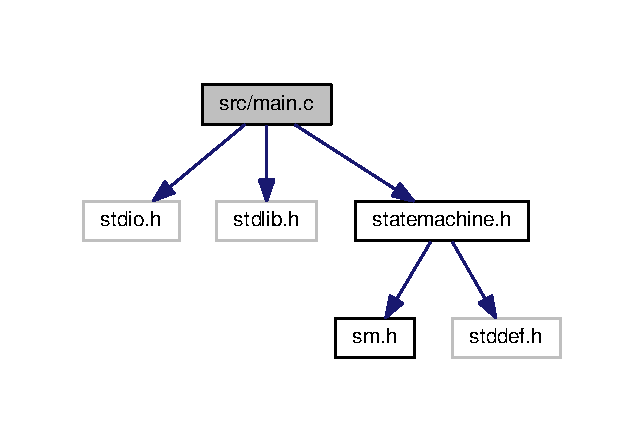
\includegraphics[width=309pt]{main_8c__incl}
\end{center}
\end{figure}
\subsubsection*{Functions}
\begin{DoxyCompactItemize}
\item 
int \hyperlink{main_8c_a840291bc02cba5474a4cb46a9b9566fe}{main} (void)
\begin{DoxyCompactList}\small\item\em Main entry point. \end{DoxyCompactList}\end{DoxyCompactItemize}


\subsubsection{Detailed Description}
Main entry point of application. 

\begin{DoxyCopyright}{Copyright}
Copyright (c) 2013, \href{mailto:marco@bacchi.at}{\tt marco@bacchi.\+at} All rights reserved.
\end{DoxyCopyright}
Redistribution and use in source and binary forms, with or without modification, are permitted provided that the following conditions are met\+:
\begin{DoxyEnumerate}
\item Redistributions of source code must retain the above copyright notice, this list of conditions and the following disclaimer.
\item Redistributions in binary form must reproduce the above copyright notice, this list of conditions and the following disclaimer in the documentation and/or other materials provided with the distribution.
\item The name of the author may not be used to endorse or promote products derived from this software without specific prior written permission.
\end{DoxyEnumerate}

T\+H\+IS S\+O\+F\+T\+W\+A\+RE IS P\+R\+O\+V\+I\+D\+ED BY T\+HE A\+U\+T\+H\+OR ``\+AS IS\textquotesingle{}\textquotesingle{} A\+ND A\+NY E\+X\+P\+R\+E\+SS OR I\+M\+P\+L\+I\+ED W\+A\+R\+R\+A\+N\+T\+I\+ES, I\+N\+C\+L\+U\+D\+I\+NG, B\+UT N\+OT L\+I\+M\+I\+T\+ED TO, T\+HE I\+M\+P\+L\+I\+ED W\+A\+R\+R\+A\+N\+T\+I\+ES OF M\+E\+R\+C\+H\+A\+N\+T\+A\+B\+I\+L\+I\+TY A\+ND F\+I\+T\+N\+E\+SS F\+OR A P\+A\+R\+T\+I\+C\+U\+L\+AR P\+U\+R\+P\+O\+SE A\+RE D\+I\+S\+C\+L\+A\+I\+M\+ED. IN NO E\+V\+E\+NT S\+H\+A\+LL T\+HE A\+U\+T\+H\+OR BE L\+I\+A\+B\+LE F\+OR A\+NY D\+I\+R\+E\+CT, I\+N\+D\+I\+R\+E\+CT, I\+N\+C\+I\+D\+E\+N\+T\+AL, S\+P\+E\+C\+I\+AL, E\+X\+E\+M\+P\+L\+A\+RY, OR C\+O\+N\+S\+E\+Q\+U\+E\+N\+T\+I\+AL D\+A\+M\+A\+G\+ES (I\+N\+C\+L\+U\+D\+I\+NG, B\+UT N\+OT L\+I\+M\+I\+T\+ED TO, P\+R\+O\+C\+U\+R\+E\+M\+E\+NT OF S\+U\+B\+S\+T\+I\+T\+U\+TE G\+O\+O\+DS OR S\+E\+R\+V\+I\+C\+ES; L\+O\+SS OF U\+SE, D\+A\+TA, OR P\+R\+O\+F\+I\+TS; OR B\+U\+S\+I\+N\+E\+SS I\+N\+T\+E\+R\+R\+U\+P\+T\+I\+ON) H\+O\+W\+E\+V\+ER C\+A\+U\+S\+ED A\+ND ON A\+NY T\+H\+E\+O\+RY OF L\+I\+A\+B\+I\+L\+I\+TY, W\+H\+E\+T\+H\+ER IN C\+O\+N\+T\+R\+A\+CT, S\+T\+R\+I\+CT L\+I\+A\+B\+I\+L\+I\+TY, OR T\+O\+RT (I\+N\+C\+L\+U\+D\+I\+NG N\+E\+G\+L\+I\+G\+E\+N\+CE OR O\+T\+H\+E\+R\+W\+I\+SE) A\+R\+I\+S\+I\+NG IN A\+NY W\+AY O\+UT OF T\+HE U\+SE OF T\+H\+IS S\+O\+F\+T\+W\+A\+RE, E\+V\+EN IF A\+D\+V\+I\+S\+ED OF T\+HE P\+O\+S\+S\+I\+B\+I\+L\+I\+TY OF S\+U\+CH D\+A\+M\+A\+GE.

\begin{DoxyVersion}{Version}
0000 
\end{DoxyVersion}
\begin{DoxyAuthor}{Authors}
\href{mailto:marco@bacchi.at}{\tt marco@bacchi.\+at} 
\end{DoxyAuthor}
\begin{DoxyDate}{Date}
2013
\end{DoxyDate}
Test Application for testing purposes during development. Has to be replaced with a unittest

{\bfseries Changelist}

\tabulinesep=1mm
\begin{longtabu} spread 0pt [c]{*4{|X[-1]}|}
\hline
\rowcolor{\tableheadbgcolor}{\bf Revision}&{\bf Date }&{\bf Name }&{\bf Change  }\\\cline{1-4}
\endfirsthead
\hline
\endfoot
\hline
\rowcolor{\tableheadbgcolor}{\bf Revision}&{\bf Date }&{\bf Name }&{\bf Change  }\\\cline{1-4}
\endhead
0000 &00.\+00.\+00&bacmar&Detailed Change Text \\\cline{1-4}
\end{longtabu}


\subsubsection{Function Documentation}
\index{main.\+c@{main.\+c}!main@{main}}
\index{main@{main}!main.\+c@{main.\+c}}
\paragraph[{\texorpdfstring{main(void)}{main(void)}}]{\setlength{\rightskip}{0pt plus 5cm}int main (
\begin{DoxyParamCaption}
\item[{void}]{}
\end{DoxyParamCaption}
)}\hypertarget{main_8c_a840291bc02cba5474a4cb46a9b9566fe}{}\label{main_8c_a840291bc02cba5474a4cb46a9b9566fe}


Main entry point. 

Initializes a designed and implemented statemachine with its initial state. Gets input from keyboard and forwards it as event to the statemachine. Valid events are from a to e.

\begin{DoxyReturn}{Returns}
E\+X\+I\+T\+\_\+\+S\+U\+C\+C\+E\+SS in case of success. Otherwise E\+X\+I\+T\+\_\+\+F\+A\+I\+L\+U\+RE. 
\end{DoxyReturn}


Definition at line 62 of file main.\+c.



Here is the call graph for this function\+:\nopagebreak
\begin{figure}[H]
\begin{center}
\leavevmode
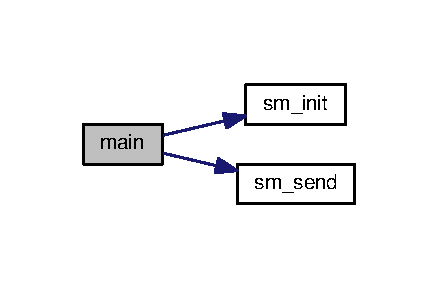
\includegraphics[width=210pt]{main_8c_a840291bc02cba5474a4cb46a9b9566fe_cgraph}
\end{center}
\end{figure}



\hypertarget{sm_8c}{}\subsection{src/sm.c File Reference}
\label{sm_8c}\index{src/sm.\+c@{src/sm.\+c}}


General U\+ML state machine implementation.  


{\ttfamily \#include \char`\"{}sm.\+h\char`\"{}}\\*
{\ttfamily \#include $<$stddef.\+h$>$}\\*
Include dependency graph for sm.\+c\+:\nopagebreak
\begin{figure}[H]
\begin{center}
\leavevmode
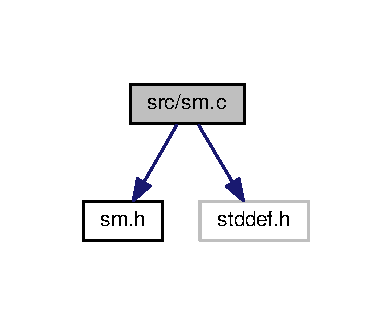
\includegraphics[width=188pt]{sm_8c__incl}
\end{center}
\end{figure}
\subsubsection*{Functions}
\begin{DoxyCompactItemize}
\item 
\hyperlink{structsm__state__t}{sm\+\_\+state\+\_\+t} $\ast$ \hyperlink{group___sm_interface_ga4d433df4f0fbd1033d3815ad870cdc5f}{sm\+\_\+init} (\hyperlink{structsm__t}{sm\+\_\+t} $\ast$sm, const \hyperlink{structsm__state__t}{sm\+\_\+state\+\_\+t} $\ast$state)
\begin{DoxyCompactList}\small\item\em Initialize a statemachine with a provided initial state. \end{DoxyCompactList}\item 
void \hyperlink{group___sm_interface_ga4a0ade9dfadc3d8a476cd64934ee369c}{sm\+\_\+terminate} (\hyperlink{structsm__t}{sm\+\_\+t} $\ast$sm)
\begin{DoxyCompactList}\small\item\em Terminates the statemachine. \end{DoxyCompactList}\item 
\hyperlink{structsm__state__t}{sm\+\_\+state\+\_\+t} $\ast$ \hyperlink{group___sm_interface_gac4c2466939ae8d63448dc84848abb7fe}{sm\+\_\+send} (\hyperlink{structsm__t}{sm\+\_\+t} $\ast$sm, \hyperlink{sm_8h_a1db78734760bf970c329945446b28432}{event\+\_\+t} event, void $\ast$data)
\begin{DoxyCompactList}\small\item\em Sends an event to a statemachine. \end{DoxyCompactList}\end{DoxyCompactItemize}
\subsubsection*{Variables}
\begin{DoxyCompactItemize}
\item 
\hyperlink{sm_8h_a858adebebe4f5a481688f24fcbbd5544}{sm\+\_\+transition\+\_\+effect\+\_\+fp} \hyperlink{sm_8c_a96c99a5af0b8720710e99939364da3af}{sm\+\_\+transition\+\_\+effect} = N\+U\+LL
\begin{DoxyCompactList}\small\item\em Action to carry out in case of a specific transition. \end{DoxyCompactList}\end{DoxyCompactItemize}


\subsubsection{Detailed Description}
General U\+ML state machine implementation. 

\begin{DoxyCopyright}{Copyright}
Copyright (c) 2013, \href{mailto:marco@bacchi.at}{\tt marco@bacchi.\+at} All rights reserved.
\end{DoxyCopyright}
Redistribution and use in source and binary forms, with or without modification, are permitted provided that the following conditions are met\+:
\begin{DoxyEnumerate}
\item Redistributions of source code must retain the above copyright notice, this list of conditions and the following disclaimer.
\item Redistributions in binary form must reproduce the above copyright notice, this list of conditions and the following disclaimer in the documentation and/or other materials provided with the distribution.
\item The name of the author may not be used to endorse or promote products derived from this software without specific prior written permission.
\end{DoxyEnumerate}

T\+H\+IS S\+O\+F\+T\+W\+A\+RE IS P\+R\+O\+V\+I\+D\+ED BY T\+HE A\+U\+T\+H\+OR ``\+AS IS\textquotesingle{}\textquotesingle{} A\+ND A\+NY E\+X\+P\+R\+E\+SS OR I\+M\+P\+L\+I\+ED W\+A\+R\+R\+A\+N\+T\+I\+ES, I\+N\+C\+L\+U\+D\+I\+NG, B\+UT N\+OT L\+I\+M\+I\+T\+ED TO, T\+HE I\+M\+P\+L\+I\+ED W\+A\+R\+R\+A\+N\+T\+I\+ES OF M\+E\+R\+C\+H\+A\+N\+T\+A\+B\+I\+L\+I\+TY A\+ND F\+I\+T\+N\+E\+SS F\+OR A P\+A\+R\+T\+I\+C\+U\+L\+AR P\+U\+R\+P\+O\+SE A\+RE D\+I\+S\+C\+L\+A\+I\+M\+ED. IN NO E\+V\+E\+NT S\+H\+A\+LL T\+HE A\+U\+T\+H\+OR BE L\+I\+A\+B\+LE F\+OR A\+NY D\+I\+R\+E\+CT, I\+N\+D\+I\+R\+E\+CT, I\+N\+C\+I\+D\+E\+N\+T\+AL, S\+P\+E\+C\+I\+AL, E\+X\+E\+M\+P\+L\+A\+RY, OR C\+O\+N\+S\+E\+Q\+U\+E\+N\+T\+I\+AL D\+A\+M\+A\+G\+ES (I\+N\+C\+L\+U\+D\+I\+NG, B\+UT N\+OT L\+I\+M\+I\+T\+ED TO, P\+R\+O\+C\+U\+R\+E\+M\+E\+NT OF S\+U\+B\+S\+T\+I\+T\+U\+TE G\+O\+O\+DS OR S\+E\+R\+V\+I\+C\+ES; L\+O\+SS OF U\+SE, D\+A\+TA, OR P\+R\+O\+F\+I\+TS; OR B\+U\+S\+I\+N\+E\+SS I\+N\+T\+E\+R\+R\+U\+P\+T\+I\+ON) H\+O\+W\+E\+V\+ER C\+A\+U\+S\+ED A\+ND ON A\+NY T\+H\+E\+O\+RY OF L\+I\+A\+B\+I\+L\+I\+TY, W\+H\+E\+T\+H\+ER IN C\+O\+N\+T\+R\+A\+CT, S\+T\+R\+I\+CT L\+I\+A\+B\+I\+L\+I\+TY, OR T\+O\+RT (I\+N\+C\+L\+U\+D\+I\+NG N\+E\+G\+L\+I\+G\+E\+N\+CE OR O\+T\+H\+E\+R\+W\+I\+SE) A\+R\+I\+S\+I\+NG IN A\+NY W\+AY O\+UT OF T\+HE U\+SE OF T\+H\+IS S\+O\+F\+T\+W\+A\+RE, E\+V\+EN IF A\+D\+V\+I\+S\+ED OF T\+HE P\+O\+S\+S\+I\+B\+I\+L\+I\+TY OF S\+U\+CH D\+A\+M\+A\+GE.

\begin{DoxyVersion}{Version}
0000 
\end{DoxyVersion}
\begin{DoxyAuthor}{Authors}
\href{mailto:marco@bacchi.at}{\tt marco@bacchi.\+at} 
\end{DoxyAuthor}
\begin{DoxyDate}{Date}
2013
\end{DoxyDate}
U\+ML state machine, also known as U\+ML state chart, is a significantly enhanced realization of the mathematical concept of a finite automaton in computer science applications as expressed in the Unified Modeling Language (U\+ML) notation. (wikipedia)~\newline
~\newline
 The concepts behind it are about organizing the way a device, computer program, or other (often technical) process works such that an entity or each of its sub-\/entities is always in exactly one of a number of possible states and where there are well-\/defined conditional transitions between these states. (wikipedia)~\newline
~\newline
 This module and its interface provides the general implementation part for any state machine written for this implementation.

This implementation supports\+:~\newline
~\newline

\begin{DoxyItemize}
\item finite flat state machines
\item guard conditions for transitions
\item state entry and exit actions
\item do actions by starting/stopping (proto)threads in entry/exit action respectively
\item transition effects (actions directly associated with a specific transition)
\end{DoxyItemize}

Limitations of this implementation\+: ~\newline
~\newline

\begin{DoxyItemize}
\item not interrupt/thread safe
\item hierarchical state machines not supported
\item execution time overhead due to generalization in comparison to quick and dirty F\+S\+Ms
\item transition fork/join not supported
\item history states not supported
\item sending events in entry/exit/transition/effect functions not allowed (due to recursion)
\end{DoxyItemize}

References\+: I\+S\+BN 3-\/8273-\/1486-\/0 Das U\+M\+L-\/\+Benutzerhandbuch

{\bfseries Changelog}

\tabulinesep=1mm
\begin{longtabu} spread 0pt [c]{*4{|X[-1]}|}
\hline
\rowcolor{\tableheadbgcolor}{\bf Revision}&{\bf Date }&{\bf Name }&{\bf Change  }\\\cline{1-4}
\endfirsthead
\hline
\endfoot
\hline
\rowcolor{\tableheadbgcolor}{\bf Revision}&{\bf Date }&{\bf Name }&{\bf Change  }\\\cline{1-4}
\endhead
0000 &00.\+00.\+00&bacmar&Detailed Change Text \\\cline{1-4}
\end{longtabu}


\subsubsection{Variable Documentation}
\index{sm.\+c@{sm.\+c}!sm\+\_\+transition\+\_\+effect@{sm\+\_\+transition\+\_\+effect}}
\index{sm\+\_\+transition\+\_\+effect@{sm\+\_\+transition\+\_\+effect}!sm.\+c@{sm.\+c}}
\paragraph[{\texorpdfstring{sm\+\_\+transition\+\_\+effect}{sm_transition_effect}}]{\setlength{\rightskip}{0pt plus 5cm}{\bf sm\+\_\+transition\+\_\+effect\+\_\+fp} sm\+\_\+transition\+\_\+effect = N\+U\+LL}\hypertarget{sm_8c_a96c99a5af0b8720710e99939364da3af}{}\label{sm_8c_a96c99a5af0b8720710e99939364da3af}


Action to carry out in case of a specific transition. 

Callback function type for transition effects.

You can associate a transition with an effect, which is an optional activity performed when a specific transition fires. The associated function may only be set within a transition function. It will be reset to N\+U\+LL again after state transition. Transition effects will not work for internal state transitions.

\begin{DoxyRemark}{Remarks}
Move to sm instance in future (for future thread safe version) or to transition function as parameter 
\end{DoxyRemark}


Definition at line 93 of file sm.\+c.


\hypertarget{sm_8h}{}\subsection{src/sm.h File Reference}
\label{sm_8h}\index{src/sm.\+h@{src/sm.\+h}}


General U\+ML state machine interface.  


This graph shows which files directly or indirectly include this file\+:\nopagebreak
\begin{figure}[H]
\begin{center}
\leavevmode
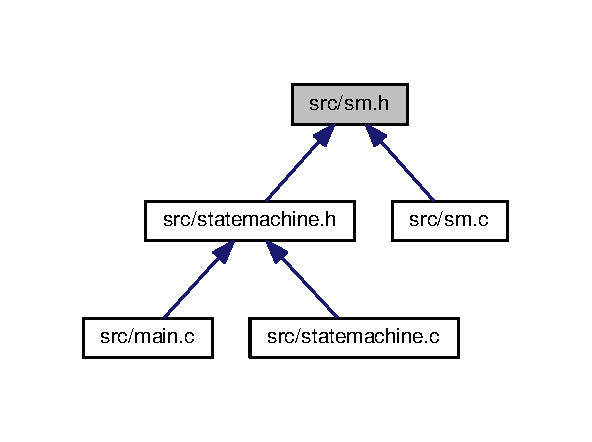
\includegraphics[width=284pt]{sm_8h__dep__incl}
\end{center}
\end{figure}
\subsubsection*{Data Structures}
\begin{DoxyCompactItemize}
\item 
struct \hyperlink{structsm__state__t}{sm\+\_\+state\+\_\+t}
\item 
struct \hyperlink{structsm__t}{sm\+\_\+t}
\begin{DoxyCompactList}\small\item\em Statemachine declaration. \end{DoxyCompactList}\end{DoxyCompactItemize}
\subsubsection*{Macros}
\begin{DoxyCompactItemize}
\item 
\#define \hyperlink{sm_8h_af833a6c202336e060a2dc2a36e0f7da5}{S\+M\+\_\+\+E\+V\+E\+N\+T\+\_\+\+I\+N\+IT}~($\sim$((\hyperlink{sm_8h_a1db78734760bf970c329945446b28432}{event\+\_\+t})0))
\item 
\#define \hyperlink{sm_8h_aff81f7c6532ee2e3c1068490df29de83}{S\+M\+\_\+\+E\+V\+E\+N\+T\+\_\+\+E\+X\+IT}~(\hyperlink{sm_8h_af833a6c202336e060a2dc2a36e0f7da5}{S\+M\+\_\+\+E\+V\+E\+N\+T\+\_\+\+I\+N\+IT}-\/1)
\item 
\#define \hyperlink{sm_8h_a052d3735a2de37a7ffea5ff2a3fcdec2}{sm\+\_\+state\+\_\+id}(base\+\_\+ptr,  state\+\_\+ptr)~((state\+\_\+ptr)-\/(base\+\_\+ptr))
\begin{DoxyCompactList}\small\item\em Preprocessor macro to retrieve state id of a state. \end{DoxyCompactList}\end{DoxyCompactItemize}
\subsubsection*{Typedefs}
\begin{DoxyCompactItemize}
\item 
typedef unsigned int \hyperlink{sm_8h_a1db78734760bf970c329945446b28432}{event\+\_\+t}
\item 
typedef struct \hyperlink{structsm__state__t}{sm\+\_\+state\+\_\+t} \hyperlink{sm_8h_a93e6a76b714190255b411b31c95490b4}{sm\+\_\+state\+\_\+t}
\item 
typedef void($\ast$ \hyperlink{sm_8h_a921fca7daf06810fad2eca72b5a0bafc}{sm\+\_\+entry\+\_\+action\+\_\+fp}) (\hyperlink{sm_8h_a1db78734760bf970c329945446b28432}{event\+\_\+t} event, void $\ast$data)
\begin{DoxyCompactList}\small\item\em Callback function type for entry actions. \end{DoxyCompactList}\item 
typedef void($\ast$ \hyperlink{sm_8h_a0b45d5fb53866f3e67285aa38b248570}{sm\+\_\+exit\+\_\+action\+\_\+fp}) (\hyperlink{sm_8h_a1db78734760bf970c329945446b28432}{event\+\_\+t} event, void $\ast$data)
\begin{DoxyCompactList}\small\item\em Callback function type for exit actions. \end{DoxyCompactList}\item 
typedef const \hyperlink{structsm__state__t}{sm\+\_\+state\+\_\+t} $\ast$($\ast$ \hyperlink{sm_8h_a48bd707c3bca2429aee6582bd67cd273}{sm\+\_\+transitions\+\_\+fp}) (\hyperlink{sm_8h_a1db78734760bf970c329945446b28432}{event\+\_\+t} event, void $\ast$data)
\begin{DoxyCompactList}\small\item\em Callback function type for transitions. \end{DoxyCompactList}\item 
typedef void($\ast$ \hyperlink{sm_8h_a858adebebe4f5a481688f24fcbbd5544}{sm\+\_\+transition\+\_\+effect\+\_\+fp}) (\hyperlink{sm_8h_a1db78734760bf970c329945446b28432}{event\+\_\+t} event, void $\ast$data)
\begin{DoxyCompactList}\small\item\em Callback function type for transition effects. \end{DoxyCompactList}\end{DoxyCompactItemize}
\subsubsection*{Functions}
\begin{DoxyCompactItemize}
\item 
\hyperlink{structsm__state__t}{sm\+\_\+state\+\_\+t} $\ast$ \hyperlink{group___sm_interface_ga4d433df4f0fbd1033d3815ad870cdc5f}{sm\+\_\+init} (\hyperlink{structsm__t}{sm\+\_\+t} $\ast$sm, const \hyperlink{structsm__state__t}{sm\+\_\+state\+\_\+t} $\ast$state)
\begin{DoxyCompactList}\small\item\em Initialize a statemachine with a provided initial state. \end{DoxyCompactList}\item 
void \hyperlink{group___sm_interface_ga4a0ade9dfadc3d8a476cd64934ee369c}{sm\+\_\+terminate} (\hyperlink{structsm__t}{sm\+\_\+t} $\ast$sm)
\begin{DoxyCompactList}\small\item\em Terminates the statemachine. \end{DoxyCompactList}\item 
\hyperlink{structsm__state__t}{sm\+\_\+state\+\_\+t} $\ast$ \hyperlink{group___sm_interface_gac4c2466939ae8d63448dc84848abb7fe}{sm\+\_\+send} (\hyperlink{structsm__t}{sm\+\_\+t} $\ast$sm, \hyperlink{sm_8h_a1db78734760bf970c329945446b28432}{event\+\_\+t} event, void $\ast$data)
\begin{DoxyCompactList}\small\item\em Sends an event to a statemachine. \end{DoxyCompactList}\end{DoxyCompactItemize}
\subsubsection*{Variables}
\begin{DoxyCompactItemize}
\item 
\hyperlink{sm_8h_a858adebebe4f5a481688f24fcbbd5544}{sm\+\_\+transition\+\_\+effect\+\_\+fp} \hyperlink{sm_8h_a96c99a5af0b8720710e99939364da3af}{sm\+\_\+transition\+\_\+effect}
\begin{DoxyCompactList}\small\item\em Callback function type for transition effects. \end{DoxyCompactList}\end{DoxyCompactItemize}


\subsubsection{Detailed Description}
General U\+ML state machine interface. 

\begin{DoxyCopyright}{Copyright}
Copyright (c) 2013, \href{mailto:marco@bacchi.at}{\tt marco@bacchi.\+at} All rights reserved.
\end{DoxyCopyright}
Redistribution and use in source and binary forms, with or without modification, are permitted provided that the following conditions are met\+:
\begin{DoxyEnumerate}
\item Redistributions of source code must retain the above copyright notice, this list of conditions and the following disclaimer.
\item Redistributions in binary form must reproduce the above copyright notice, this list of conditions and the following disclaimer in the documentation and/or other materials provided with the distribution.
\item The name of the author may not be used to endorse or promote products derived from this software without specific prior written permission.
\end{DoxyEnumerate}

T\+H\+IS S\+O\+F\+T\+W\+A\+RE IS P\+R\+O\+V\+I\+D\+ED BY T\+HE A\+U\+T\+H\+OR ``\+AS IS\textquotesingle{}\textquotesingle{} A\+ND A\+NY E\+X\+P\+R\+E\+SS OR I\+M\+P\+L\+I\+ED W\+A\+R\+R\+A\+N\+T\+I\+ES, I\+N\+C\+L\+U\+D\+I\+NG, B\+UT N\+OT L\+I\+M\+I\+T\+ED TO, T\+HE I\+M\+P\+L\+I\+ED W\+A\+R\+R\+A\+N\+T\+I\+ES OF M\+E\+R\+C\+H\+A\+N\+T\+A\+B\+I\+L\+I\+TY A\+ND F\+I\+T\+N\+E\+SS F\+OR A P\+A\+R\+T\+I\+C\+U\+L\+AR P\+U\+R\+P\+O\+SE A\+RE D\+I\+S\+C\+L\+A\+I\+M\+ED. IN NO E\+V\+E\+NT S\+H\+A\+LL T\+HE A\+U\+T\+H\+OR BE L\+I\+A\+B\+LE F\+OR A\+NY D\+I\+R\+E\+CT, I\+N\+D\+I\+R\+E\+CT, I\+N\+C\+I\+D\+E\+N\+T\+AL, S\+P\+E\+C\+I\+AL, E\+X\+E\+M\+P\+L\+A\+RY, OR C\+O\+N\+S\+E\+Q\+U\+E\+N\+T\+I\+AL D\+A\+M\+A\+G\+ES (I\+N\+C\+L\+U\+D\+I\+NG, B\+UT N\+OT L\+I\+M\+I\+T\+ED TO, P\+R\+O\+C\+U\+R\+E\+M\+E\+NT OF S\+U\+B\+S\+T\+I\+T\+U\+TE G\+O\+O\+DS OR S\+E\+R\+V\+I\+C\+ES; L\+O\+SS OF U\+SE, D\+A\+TA, OR P\+R\+O\+F\+I\+TS; OR B\+U\+S\+I\+N\+E\+SS I\+N\+T\+E\+R\+R\+U\+P\+T\+I\+ON) H\+O\+W\+E\+V\+ER C\+A\+U\+S\+ED A\+ND ON A\+NY T\+H\+E\+O\+RY OF L\+I\+A\+B\+I\+L\+I\+TY, W\+H\+E\+T\+H\+ER IN C\+O\+N\+T\+R\+A\+CT, S\+T\+R\+I\+CT L\+I\+A\+B\+I\+L\+I\+TY, OR T\+O\+RT (I\+N\+C\+L\+U\+D\+I\+NG N\+E\+G\+L\+I\+G\+E\+N\+CE OR O\+T\+H\+E\+R\+W\+I\+SE) A\+R\+I\+S\+I\+NG IN A\+NY W\+AY O\+UT OF T\+HE U\+SE OF T\+H\+IS S\+O\+F\+T\+W\+A\+RE, E\+V\+EN IF A\+D\+V\+I\+S\+ED OF T\+HE P\+O\+S\+S\+I\+B\+I\+L\+I\+TY OF S\+U\+CH D\+A\+M\+A\+GE.

\begin{DoxyVersion}{Version}
0000 
\end{DoxyVersion}
\begin{DoxyAuthor}{Authors}
\href{mailto:marco@bacchi.at}{\tt marco@bacchi.\+at} 
\end{DoxyAuthor}
\begin{DoxyDate}{Date}
2013
\end{DoxyDate}
U\+ML state machine, also known as U\+ML state chart, is a significantly enhanced realization of the mathematical concept of a finite automaton in computer science applications as expressed in the Unified Modeling Language (U\+ML) notation. (wikipedia)~\newline
~\newline
 The concepts behind it are about organizing the way a device, computer program, or other (often technical) process works such that an entity or each of its sub-\/entities is always in exactly one of a number of possible states and where there are well-\/defined conditional transitions between these states. (wikipedia)~\newline
~\newline
 This module and its interface provides the general implementation part for any state machine written for this implementation.

This implementation supports\+:~\newline
~\newline

\begin{DoxyItemize}
\item finite flat state machines
\item guard conditions for transitions
\item state entry and exit actions
\item do actions by starting/stopping (proto)threads in entry/exit action respectively
\item transition effects (actions directly associated with a specific transition)
\end{DoxyItemize}

Limitations of this implementation\+: ~\newline
~\newline

\begin{DoxyItemize}
\item not interrupt/thread safe
\item hierarchical state machines not supported
\item execution time overhead due to generalization in comparison to quick and dirty F\+S\+Ms
\item transition fork/join not supported
\item history states not supported
\item sending events in entry/exit/transition/effect functions not allowed (due to recursion)
\end{DoxyItemize}

{\bfseries Changelog}

\tabulinesep=1mm
\begin{longtabu} spread 0pt [c]{*4{|X[-1]}|}
\hline
\rowcolor{\tableheadbgcolor}{\bf Revision}&{\bf Date }&{\bf Name }&{\bf Change  }\\\cline{1-4}
\endfirsthead
\hline
\endfoot
\hline
\rowcolor{\tableheadbgcolor}{\bf Revision}&{\bf Date }&{\bf Name }&{\bf Change  }\\\cline{1-4}
\endhead
0000 &00.\+00.\+00&bacmar&Detailed Change Text \\\cline{1-4}
\end{longtabu}
References\+: I\+S\+BN 3-\/8273-\/1486-\/0 Das U\+M\+L-\/\+Benutzerhandbuch 

\subsubsection{Macro Definition Documentation}
\index{sm.\+h@{sm.\+h}!S\+M\+\_\+\+E\+V\+E\+N\+T\+\_\+\+E\+X\+IT@{S\+M\+\_\+\+E\+V\+E\+N\+T\+\_\+\+E\+X\+IT}}
\index{S\+M\+\_\+\+E\+V\+E\+N\+T\+\_\+\+E\+X\+IT@{S\+M\+\_\+\+E\+V\+E\+N\+T\+\_\+\+E\+X\+IT}!sm.\+h@{sm.\+h}}
\paragraph[{\texorpdfstring{S\+M\+\_\+\+E\+V\+E\+N\+T\+\_\+\+E\+X\+IT}{SM_EVENT_EXIT}}]{\setlength{\rightskip}{0pt plus 5cm}\#define S\+M\+\_\+\+E\+V\+E\+N\+T\+\_\+\+E\+X\+IT~({\bf S\+M\+\_\+\+E\+V\+E\+N\+T\+\_\+\+I\+N\+IT}-\/1)}\hypertarget{sm_8h_aff81f7c6532ee2e3c1068490df29de83}{}\label{sm_8h_aff81f7c6532ee2e3c1068490df29de83}
Definition of event id to terminate a statemachine, must not be sent by the user 

Definition at line 83 of file sm.\+h.

\index{sm.\+h@{sm.\+h}!S\+M\+\_\+\+E\+V\+E\+N\+T\+\_\+\+I\+N\+IT@{S\+M\+\_\+\+E\+V\+E\+N\+T\+\_\+\+I\+N\+IT}}
\index{S\+M\+\_\+\+E\+V\+E\+N\+T\+\_\+\+I\+N\+IT@{S\+M\+\_\+\+E\+V\+E\+N\+T\+\_\+\+I\+N\+IT}!sm.\+h@{sm.\+h}}
\paragraph[{\texorpdfstring{S\+M\+\_\+\+E\+V\+E\+N\+T\+\_\+\+I\+N\+IT}{SM_EVENT_INIT}}]{\setlength{\rightskip}{0pt plus 5cm}\#define S\+M\+\_\+\+E\+V\+E\+N\+T\+\_\+\+I\+N\+IT~($\sim$(({\bf event\+\_\+t})0))}\hypertarget{sm_8h_af833a6c202336e060a2dc2a36e0f7da5}{}\label{sm_8h_af833a6c202336e060a2dc2a36e0f7da5}
Definition of event id to initialize a statemachine, must not be sent by the user 

Definition at line 81 of file sm.\+h.

\index{sm.\+h@{sm.\+h}!sm\+\_\+state\+\_\+id@{sm\+\_\+state\+\_\+id}}
\index{sm\+\_\+state\+\_\+id@{sm\+\_\+state\+\_\+id}!sm.\+h@{sm.\+h}}
\paragraph[{\texorpdfstring{sm\+\_\+state\+\_\+id}{sm_state_id}}]{\setlength{\rightskip}{0pt plus 5cm}\#define sm\+\_\+state\+\_\+id(
\begin{DoxyParamCaption}
\item[{}]{base\+\_\+ptr, }
\item[{}]{state\+\_\+ptr}
\end{DoxyParamCaption}
)~((state\+\_\+ptr)-\/(base\+\_\+ptr))}\hypertarget{sm_8h_a052d3735a2de37a7ffea5ff2a3fcdec2}{}\label{sm_8h_a052d3735a2de37a7ffea5ff2a3fcdec2}


Preprocessor macro to retrieve state id of a state. 

Preprocessor macro to retrieve state id of a state.


\begin{DoxyParams}[1]{Parameters}
\mbox{\tt in}  & {\em base\+\_\+ptr} & Pointer to the state table \\
\hline
\mbox{\tt in}  & {\em state\+\_\+ptr} & Pointer to a specific state of the state table\\
\hline
\end{DoxyParams}
\begin{DoxyReturn}{Returns}
id of the specific state 
\end{DoxyReturn}


Definition at line 190 of file sm.\+h.



\subsubsection{Typedef Documentation}
\index{sm.\+h@{sm.\+h}!event\+\_\+t@{event\+\_\+t}}
\index{event\+\_\+t@{event\+\_\+t}!sm.\+h@{sm.\+h}}
\paragraph[{\texorpdfstring{event\+\_\+t}{event_t}}]{\setlength{\rightskip}{0pt plus 5cm}typedef unsigned int {\bf event\+\_\+t}}\hypertarget{sm_8h_a1db78734760bf970c329945446b28432}{}\label{sm_8h_a1db78734760bf970c329945446b28432}
An event is something that happens that affects the system. An event can have associated parameters, allowing the event instance to convey not only the occurrence of some interesting incident but also quantitative information regarding that occurrence. The associated parameters can be forwarded to the state machine via the data pointer of the sm\+\_\+send function 

Definition at line 92 of file sm.\+h.

\index{sm.\+h@{sm.\+h}!sm\+\_\+entry\+\_\+action\+\_\+fp@{sm\+\_\+entry\+\_\+action\+\_\+fp}}
\index{sm\+\_\+entry\+\_\+action\+\_\+fp@{sm\+\_\+entry\+\_\+action\+\_\+fp}!sm.\+h@{sm.\+h}}
\paragraph[{\texorpdfstring{sm\+\_\+entry\+\_\+action\+\_\+fp}{sm_entry_action_fp}}]{\setlength{\rightskip}{0pt plus 5cm}typedef void($\ast$ sm\+\_\+entry\+\_\+action\+\_\+fp) ({\bf event\+\_\+t} event, void $\ast$data)}\hypertarget{sm_8h_a921fca7daf06810fad2eca72b5a0bafc}{}\label{sm_8h_a921fca7daf06810fad2eca72b5a0bafc}


Callback function type for entry actions. 

Every state in a U\+ML state chart can have an optional entry action, which is executed upon entry to a state. Entry actions are associated with states, not transitions. Regardless of how a state is entered, its entry action will be executed.


\begin{DoxyParams}{Parameters}
{\em event} & Triggering event \\
\hline
{\em data} & Data associated with the event \\
\hline
\end{DoxyParams}


Definition at line 110 of file sm.\+h.

\index{sm.\+h@{sm.\+h}!sm\+\_\+exit\+\_\+action\+\_\+fp@{sm\+\_\+exit\+\_\+action\+\_\+fp}}
\index{sm\+\_\+exit\+\_\+action\+\_\+fp@{sm\+\_\+exit\+\_\+action\+\_\+fp}!sm.\+h@{sm.\+h}}
\paragraph[{\texorpdfstring{sm\+\_\+exit\+\_\+action\+\_\+fp}{sm_exit_action_fp}}]{\setlength{\rightskip}{0pt plus 5cm}typedef void($\ast$ sm\+\_\+exit\+\_\+action\+\_\+fp) ({\bf event\+\_\+t} event, void $\ast$data)}\hypertarget{sm_8h_a0b45d5fb53866f3e67285aa38b248570}{}\label{sm_8h_a0b45d5fb53866f3e67285aa38b248570}


Callback function type for exit actions. 

Every state in a U\+ML state chart can have an optional exit action, which is executed upon exit from a state. Exit actions are associated with states, not transitions. Regardless of how a state is left, its exit action will be executed.


\begin{DoxyParams}{Parameters}
{\em event} & Triggering event \\
\hline
{\em data} & Data associated with the event \\
\hline
\end{DoxyParams}


Definition at line 122 of file sm.\+h.

\index{sm.\+h@{sm.\+h}!sm\+\_\+state\+\_\+t@{sm\+\_\+state\+\_\+t}}
\index{sm\+\_\+state\+\_\+t@{sm\+\_\+state\+\_\+t}!sm.\+h@{sm.\+h}}
\paragraph[{\texorpdfstring{sm\+\_\+state\+\_\+t}{sm_state_t}}]{\setlength{\rightskip}{0pt plus 5cm}typedef struct {\bf sm\+\_\+state\+\_\+t} {\bf sm\+\_\+state\+\_\+t}}\hypertarget{sm_8h_a93e6a76b714190255b411b31c95490b4}{}\label{sm_8h_a93e6a76b714190255b411b31c95490b4}
Forward declaration of sm\+\_\+state structure 

Definition at line 97 of file sm.\+h.

\index{sm.\+h@{sm.\+h}!sm\+\_\+transition\+\_\+effect\+\_\+fp@{sm\+\_\+transition\+\_\+effect\+\_\+fp}}
\index{sm\+\_\+transition\+\_\+effect\+\_\+fp@{sm\+\_\+transition\+\_\+effect\+\_\+fp}!sm.\+h@{sm.\+h}}
\paragraph[{\texorpdfstring{sm\+\_\+transition\+\_\+effect\+\_\+fp}{sm_transition_effect_fp}}]{\setlength{\rightskip}{0pt plus 5cm}typedef void($\ast$ sm\+\_\+transition\+\_\+effect\+\_\+fp) ({\bf event\+\_\+t} event, void $\ast$data)}\hypertarget{sm_8h_a858adebebe4f5a481688f24fcbbd5544}{}\label{sm_8h_a858adebebe4f5a481688f24fcbbd5544}


Callback function type for transition effects. 

Switching from one state to another is called state transition. An effect specifies an optional behavior to be performed when the transition fires. The transition effect has to be set in the transition function and is invoked after exit of the source state and before entry of the target state.


\begin{DoxyParams}{Parameters}
{\em event} & Triggering event \\
\hline
{\em data} & Data associated with the event \\
\hline
\end{DoxyParams}


Definition at line 149 of file sm.\+h.

\index{sm.\+h@{sm.\+h}!sm\+\_\+transitions\+\_\+fp@{sm\+\_\+transitions\+\_\+fp}}
\index{sm\+\_\+transitions\+\_\+fp@{sm\+\_\+transitions\+\_\+fp}!sm.\+h@{sm.\+h}}
\paragraph[{\texorpdfstring{sm\+\_\+transitions\+\_\+fp}{sm_transitions_fp}}]{\setlength{\rightskip}{0pt plus 5cm}typedef const {\bf sm\+\_\+state\+\_\+t}$\ast$($\ast$ sm\+\_\+transitions\+\_\+fp) ({\bf event\+\_\+t} event, void $\ast$data)}\hypertarget{sm_8h_a48bd707c3bca2429aee6582bd67cd273}{}\label{sm_8h_a48bd707c3bca2429aee6582bd67cd273}


Callback function type for transitions. 

Switching from one state to another is called state transition, and the event that causes it is called the triggering event, or simply the trigger. This function has to be implemented by the state machine designer for each state of the state machine.


\begin{DoxyParams}{Parameters}
{\em event} & Triggering event \\
\hline
{\em data} & Data associated with the event\\
\hline
\end{DoxyParams}
\begin{DoxyReturn}{Returns}
New state in case of external transition. Same state as before in case of self transition. N\+U\+LL in case of internal or no transition. 
\end{DoxyReturn}


Definition at line 137 of file sm.\+h.



\subsubsection{Variable Documentation}
\index{sm.\+h@{sm.\+h}!sm\+\_\+transition\+\_\+effect@{sm\+\_\+transition\+\_\+effect}}
\index{sm\+\_\+transition\+\_\+effect@{sm\+\_\+transition\+\_\+effect}!sm.\+h@{sm.\+h}}
\paragraph[{\texorpdfstring{sm\+\_\+transition\+\_\+effect}{sm_transition_effect}}]{\setlength{\rightskip}{0pt plus 5cm}{\bf sm\+\_\+transition\+\_\+effect\+\_\+fp} sm\+\_\+transition\+\_\+effect}\hypertarget{sm_8h_a96c99a5af0b8720710e99939364da3af}{}\label{sm_8h_a96c99a5af0b8720710e99939364da3af}


Callback function type for transition effects. 

Specifies an optional behavior to be performed when the transition fires.\+global variable for the transition effect

Callback function type for transition effects.

You can associate a transition with an effect, which is an optional activity performed when a specific transition fires. The associated function may only be set within a transition function. It will be reset to N\+U\+LL again after state transition. Transition effects will not work for internal state transitions.

\begin{DoxyRemark}{Remarks}
Move to sm instance in future (for future thread safe version) or to transition function as parameter 
\end{DoxyRemark}


Definition at line 93 of file sm.\+c.


\hypertarget{statemachine_8c}{}\subsection{src/statemachine.c File Reference}
\label{statemachine_8c}\index{src/statemachine.\+c@{src/statemachine.\+c}}


Statemachine for testing purposes -\/ implementation.  


{\ttfamily \#include \char`\"{}statemachine.\+h\char`\"{}}\\*
{\ttfamily \#include $<$stdbool.\+h$>$}\\*
{\ttfamily \#include $<$stdio.\+h$>$}\\*
Include dependency graph for statemachine.\+c\+:\nopagebreak
\begin{figure}[H]
\begin{center}
\leavevmode
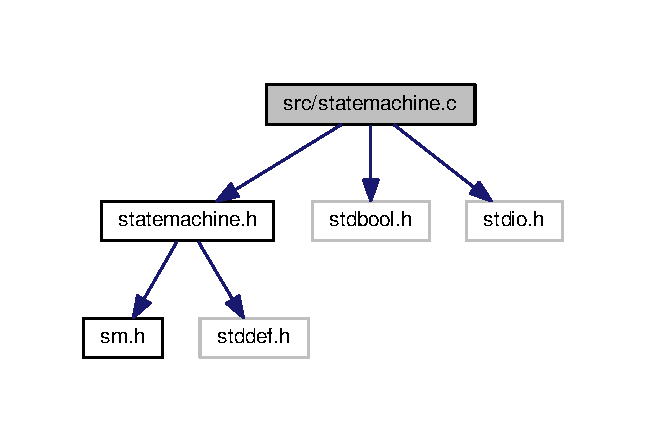
\includegraphics[width=310pt]{statemachine_8c__incl}
\end{center}
\end{figure}
\subsubsection*{Macros}
\begin{DoxyCompactItemize}
\item 
\#define \hyperlink{statemachine_8c_ad72dbcf6d0153db1b8d8a58001feed83}{D\+E\+B\+UG}~1
\item 
\#define \hyperlink{statemachine_8c_ae8924623ca601364965e3d88fb7f40fa}{D\+BG}(...)~printf(\+\_\+\+\_\+\+V\+A\+\_\+\+A\+R\+G\+S\+\_\+\+\_\+)
\end{DoxyCompactItemize}
\subsubsection*{Functions}
\begin{DoxyCompactItemize}
\item 
void \hyperlink{statemachine_8c_a19575b4361bd5f13002ea2a60abee30e}{A\+\_\+entry} (\hyperlink{sm_8h_a1db78734760bf970c329945446b28432}{event\+\_\+t} event, void $\ast$data)
\begin{DoxyCompactList}\small\item\em State A entry function. \end{DoxyCompactList}\item 
const \hyperlink{structsm__state__t}{sm\+\_\+state\+\_\+t} $\ast$ \hyperlink{statemachine_8c_aed25a8dc0c3a7fbe99cb1df00c906308}{A\+\_\+transitions} (\hyperlink{sm_8h_a1db78734760bf970c329945446b28432}{event\+\_\+t} event, void $\ast$data)
\begin{DoxyCompactList}\small\item\em State A transitions function. \end{DoxyCompactList}\item 
void \hyperlink{statemachine_8c_a6d1d85f00f8d214d50928143924360e8}{A\+\_\+exit} (\hyperlink{sm_8h_a1db78734760bf970c329945446b28432}{event\+\_\+t} event, void $\ast$data)
\begin{DoxyCompactList}\small\item\em State A exit function. \end{DoxyCompactList}\item 
void \hyperlink{statemachine_8c_a6ee1fe17283b4adb8113f6758ebe126f}{Be\+C\+\_\+transition\+\_\+effect} (\hyperlink{sm_8h_a1db78734760bf970c329945446b28432}{event\+\_\+t} event, void $\ast$data)
\item 
const \hyperlink{structsm__state__t}{sm\+\_\+state\+\_\+t} $\ast$ \hyperlink{statemachine_8c_aa9f36d192c7bb00314ac80a8d2df48a9}{B\+\_\+transitions} (\hyperlink{sm_8h_a1db78734760bf970c329945446b28432}{event\+\_\+t} event, void $\ast$data)
\begin{DoxyCompactList}\small\item\em State B transitions function. \end{DoxyCompactList}\item 
void \hyperlink{statemachine_8c_a9268b737532961b741afe6d16b6b27d6}{B\+\_\+exit} (\hyperlink{sm_8h_a1db78734760bf970c329945446b28432}{event\+\_\+t} event, void $\ast$data)
\begin{DoxyCompactList}\small\item\em State B exit function. \end{DoxyCompactList}\item 
void \hyperlink{statemachine_8c_ab162221c19b71005e9f3b2d5bed511e2}{C\+\_\+entry} (\hyperlink{sm_8h_a1db78734760bf970c329945446b28432}{event\+\_\+t} event, void $\ast$data)
\begin{DoxyCompactList}\small\item\em State C entry function. \end{DoxyCompactList}\item 
const \hyperlink{structsm__state__t}{sm\+\_\+state\+\_\+t} $\ast$ \hyperlink{statemachine_8c_a7c2e65f9b16175c058af547044882809}{C\+\_\+transitions} (\hyperlink{sm_8h_a1db78734760bf970c329945446b28432}{event\+\_\+t} event, void $\ast$data)
\begin{DoxyCompactList}\small\item\em State C transitions function. \end{DoxyCompactList}\end{DoxyCompactItemize}
\subsubsection*{Variables}
\begin{DoxyCompactItemize}
\item 
bool \hyperlink{statemachine_8c_a7f7d42bd83a62658be38736703dda051}{guard} = false
\item 
const \hyperlink{structsm__state__t}{sm\+\_\+state\+\_\+t} \hyperlink{statemachine_8c_aa017019d16cc39ebd231a5f2598d79c0}{statemachine\+\_\+states} \mbox{[}$\,$\mbox{]}
\item 
const size\+\_\+t \hyperlink{statemachine_8c_a03b8b76d23b4f034c554518a79c91e7e}{statemachine\+\_\+state\+\_\+count} = sizeof(\hyperlink{statemachine_8h_aa017019d16cc39ebd231a5f2598d79c0}{statemachine\+\_\+states})/sizeof(\hyperlink{statemachine_8h_aa017019d16cc39ebd231a5f2598d79c0}{statemachine\+\_\+states}\mbox{[}0\mbox{]})
\end{DoxyCompactItemize}


\subsubsection{Detailed Description}
Statemachine for testing purposes -\/ implementation. 

\begin{DoxyCopyright}{Copyright}
Copyright (c) 2013, \href{mailto:marco@bacchi.at}{\tt marco@bacchi.\+at} All rights reserved.
\end{DoxyCopyright}
Redistribution and use in source and binary forms, with or without modification, are permitted provided that the following conditions are met\+:
\begin{DoxyEnumerate}
\item Redistributions of source code must retain the above copyright notice, this list of conditions and the following disclaimer.
\item Redistributions in binary form must reproduce the above copyright notice, this list of conditions and the following disclaimer in the documentation and/or other materials provided with the distribution.
\item The name of the author may not be used to endorse or promote products derived from this software without specific prior written permission.
\end{DoxyEnumerate}

T\+H\+IS S\+O\+F\+T\+W\+A\+RE IS P\+R\+O\+V\+I\+D\+ED BY T\+HE A\+U\+T\+H\+OR ``\+AS IS\textquotesingle{}\textquotesingle{} A\+ND A\+NY E\+X\+P\+R\+E\+SS OR I\+M\+P\+L\+I\+ED W\+A\+R\+R\+A\+N\+T\+I\+ES, I\+N\+C\+L\+U\+D\+I\+NG, B\+UT N\+OT L\+I\+M\+I\+T\+ED TO, T\+HE I\+M\+P\+L\+I\+ED W\+A\+R\+R\+A\+N\+T\+I\+ES OF M\+E\+R\+C\+H\+A\+N\+T\+A\+B\+I\+L\+I\+TY A\+ND F\+I\+T\+N\+E\+SS F\+OR A P\+A\+R\+T\+I\+C\+U\+L\+AR P\+U\+R\+P\+O\+SE A\+RE D\+I\+S\+C\+L\+A\+I\+M\+ED. IN NO E\+V\+E\+NT S\+H\+A\+LL T\+HE A\+U\+T\+H\+OR BE L\+I\+A\+B\+LE F\+OR A\+NY D\+I\+R\+E\+CT, I\+N\+D\+I\+R\+E\+CT, I\+N\+C\+I\+D\+E\+N\+T\+AL, S\+P\+E\+C\+I\+AL, E\+X\+E\+M\+P\+L\+A\+RY, OR C\+O\+N\+S\+E\+Q\+U\+E\+N\+T\+I\+AL D\+A\+M\+A\+G\+ES (I\+N\+C\+L\+U\+D\+I\+NG, B\+UT N\+OT L\+I\+M\+I\+T\+ED TO, P\+R\+O\+C\+U\+R\+E\+M\+E\+NT OF S\+U\+B\+S\+T\+I\+T\+U\+TE G\+O\+O\+DS OR S\+E\+R\+V\+I\+C\+ES; L\+O\+SS OF U\+SE, D\+A\+TA, OR P\+R\+O\+F\+I\+TS; OR B\+U\+S\+I\+N\+E\+SS I\+N\+T\+E\+R\+R\+U\+P\+T\+I\+ON) H\+O\+W\+E\+V\+ER C\+A\+U\+S\+ED A\+ND ON A\+NY T\+H\+E\+O\+RY OF L\+I\+A\+B\+I\+L\+I\+TY, W\+H\+E\+T\+H\+ER IN C\+O\+N\+T\+R\+A\+CT, S\+T\+R\+I\+CT L\+I\+A\+B\+I\+L\+I\+TY, OR T\+O\+RT (I\+N\+C\+L\+U\+D\+I\+NG N\+E\+G\+L\+I\+G\+E\+N\+CE OR O\+T\+H\+E\+R\+W\+I\+SE) A\+R\+I\+S\+I\+NG IN A\+NY W\+AY O\+UT OF T\+HE U\+SE OF T\+H\+IS S\+O\+F\+T\+W\+A\+RE, E\+V\+EN IF A\+D\+V\+I\+S\+ED OF T\+HE P\+O\+S\+S\+I\+B\+I\+L\+I\+TY OF S\+U\+CH D\+A\+M\+A\+GE.

\begin{DoxyVersion}{Version}
0000 
\end{DoxyVersion}
\begin{DoxyAuthor}{Authors}
\href{mailto:marco@bacchi.at}{\tt marco@bacchi.\+at} 
\end{DoxyAuthor}
\begin{DoxyDate}{Date}
2013
\end{DoxyDate}
This statemachine is for testing purposes. It defines three states and some testing transitions between the states. It also makes use of a guard condition and covers exit/entry actions, transition effects and internal transitions.

 
\begin{DoxyImage}
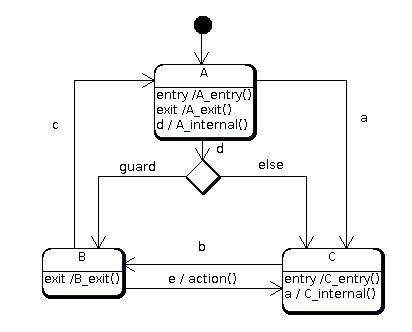
\includegraphics[width=10cm]{sm_test_statemachine.png}
\caption{Statemachine for testing purposes}
\end{DoxyImage}


{\bfseries Changelist}

\tabulinesep=1mm
\begin{longtabu} spread 0pt [c]{*4{|X[-1]}|}
\hline
\rowcolor{\tableheadbgcolor}{\bf Revision}&{\bf Date }&{\bf Name }&{\bf Change  }\\\cline{1-4}
\endfirsthead
\hline
\endfoot
\hline
\rowcolor{\tableheadbgcolor}{\bf Revision}&{\bf Date }&{\bf Name }&{\bf Change  }\\\cline{1-4}
\endhead
0000 &00.\+00.\+00&bacmar&Detailed Change Text \\\cline{1-4}
\end{longtabu}


\subsubsection{Macro Definition Documentation}
\index{statemachine.\+c@{statemachine.\+c}!D\+BG@{D\+BG}}
\index{D\+BG@{D\+BG}!statemachine.\+c@{statemachine.\+c}}
\paragraph[{\texorpdfstring{D\+BG}{DBG}}]{\setlength{\rightskip}{0pt plus 5cm}\#define D\+BG(
\begin{DoxyParamCaption}
\item[{}]{...}
\end{DoxyParamCaption}
)~printf(\+\_\+\+\_\+\+V\+A\+\_\+\+A\+R\+G\+S\+\_\+\+\_\+)}\hypertarget{statemachine_8c_ae8924623ca601364965e3d88fb7f40fa}{}\label{statemachine_8c_ae8924623ca601364965e3d88fb7f40fa}


Definition at line 58 of file statemachine.\+c.

\index{statemachine.\+c@{statemachine.\+c}!D\+E\+B\+UG@{D\+E\+B\+UG}}
\index{D\+E\+B\+UG@{D\+E\+B\+UG}!statemachine.\+c@{statemachine.\+c}}
\paragraph[{\texorpdfstring{D\+E\+B\+UG}{DEBUG}}]{\setlength{\rightskip}{0pt plus 5cm}\#define D\+E\+B\+UG~1}\hypertarget{statemachine_8c_ad72dbcf6d0153db1b8d8a58001feed83}{}\label{statemachine_8c_ad72dbcf6d0153db1b8d8a58001feed83}


Definition at line 54 of file statemachine.\+c.



\subsubsection{Function Documentation}
\index{statemachine.\+c@{statemachine.\+c}!A\+\_\+entry@{A\+\_\+entry}}
\index{A\+\_\+entry@{A\+\_\+entry}!statemachine.\+c@{statemachine.\+c}}
\paragraph[{\texorpdfstring{A\+\_\+entry(event\+\_\+t event, void $\ast$data)}{A_entry(event_t event, void *data)}}]{\setlength{\rightskip}{0pt plus 5cm}void A\+\_\+entry (
\begin{DoxyParamCaption}
\item[{{\bf event\+\_\+t}}]{event, }
\item[{void $\ast$}]{data}
\end{DoxyParamCaption}
)}\hypertarget{statemachine_8c_a19575b4361bd5f13002ea2a60abee30e}{}\label{statemachine_8c_a19575b4361bd5f13002ea2a60abee30e}


State A entry function. 

Every state in a U\+ML state chart can have an optional entry action, which is executed upon entry to a state. Entry actions are associated with states, not transitions. Regardless of how a state is entered, its entry action will be executed.


\begin{DoxyParams}{Parameters}
{\em event} & Triggering event \\
\hline
{\em data} & Data associated with the event \\
\hline
\end{DoxyParams}


Definition at line 75 of file statemachine.\+c.

\index{statemachine.\+c@{statemachine.\+c}!A\+\_\+exit@{A\+\_\+exit}}
\index{A\+\_\+exit@{A\+\_\+exit}!statemachine.\+c@{statemachine.\+c}}
\paragraph[{\texorpdfstring{A\+\_\+exit(event\+\_\+t event, void $\ast$data)}{A_exit(event_t event, void *data)}}]{\setlength{\rightskip}{0pt plus 5cm}void A\+\_\+exit (
\begin{DoxyParamCaption}
\item[{{\bf event\+\_\+t}}]{event, }
\item[{void $\ast$}]{data}
\end{DoxyParamCaption}
)}\hypertarget{statemachine_8c_a6d1d85f00f8d214d50928143924360e8}{}\label{statemachine_8c_a6d1d85f00f8d214d50928143924360e8}


State A exit function. 

Every state in a U\+ML state chart can have an optional exit action, which is executed upon exit from a state. Exit actions are associated with states, not transitions. Regardless of how a state is left, its exit action will be executed.


\begin{DoxyParams}{Parameters}
{\em event} & Triggering event \\
\hline
{\em data} & Data associated with the event \\
\hline
\end{DoxyParams}


Definition at line 123 of file statemachine.\+c.

\index{statemachine.\+c@{statemachine.\+c}!A\+\_\+transitions@{A\+\_\+transitions}}
\index{A\+\_\+transitions@{A\+\_\+transitions}!statemachine.\+c@{statemachine.\+c}}
\paragraph[{\texorpdfstring{A\+\_\+transitions(event\+\_\+t event, void $\ast$data)}{A_transitions(event_t event, void *data)}}]{\setlength{\rightskip}{0pt plus 5cm}const {\bf sm\+\_\+state\+\_\+t}$\ast$ A\+\_\+transitions (
\begin{DoxyParamCaption}
\item[{{\bf event\+\_\+t}}]{event, }
\item[{void $\ast$}]{data}
\end{DoxyParamCaption}
)}\hypertarget{statemachine_8c_aed25a8dc0c3a7fbe99cb1df00c906308}{}\label{statemachine_8c_aed25a8dc0c3a7fbe99cb1df00c906308}


State A transitions function. 

Switching from one state to another is called state transition, and the event that causes it is called the triggering event, or simply the trigger. This function has to be implemented by the state machine designer for each state of the state machine.


\begin{DoxyParams}{Parameters}
{\em event} & Triggering event \\
\hline
{\em data} & Data associated with the event\\
\hline
\end{DoxyParams}
\begin{DoxyReturn}{Returns}
New state in case of external transition. Same state as before in case of self transition. N\+U\+LL in case of internal or no transition. 
\end{DoxyReturn}


Definition at line 92 of file statemachine.\+c.

\index{statemachine.\+c@{statemachine.\+c}!B\+\_\+exit@{B\+\_\+exit}}
\index{B\+\_\+exit@{B\+\_\+exit}!statemachine.\+c@{statemachine.\+c}}
\paragraph[{\texorpdfstring{B\+\_\+exit(event\+\_\+t event, void $\ast$data)}{B_exit(event_t event, void *data)}}]{\setlength{\rightskip}{0pt plus 5cm}void B\+\_\+exit (
\begin{DoxyParamCaption}
\item[{{\bf event\+\_\+t}}]{event, }
\item[{void $\ast$}]{data}
\end{DoxyParamCaption}
)}\hypertarget{statemachine_8c_a9268b737532961b741afe6d16b6b27d6}{}\label{statemachine_8c_a9268b737532961b741afe6d16b6b27d6}


State B exit function. 

Every state in a U\+ML state chart can have an optional exit action, which is executed upon exit from a state. Exit actions are associated with states, not transitions. Regardless of how a state is left, its exit action will be executed.


\begin{DoxyParams}{Parameters}
{\em event} & Triggering event \\
\hline
{\em data} & Data associated with the event \\
\hline
\end{DoxyParams}


Definition at line 176 of file statemachine.\+c.

\index{statemachine.\+c@{statemachine.\+c}!B\+\_\+transitions@{B\+\_\+transitions}}
\index{B\+\_\+transitions@{B\+\_\+transitions}!statemachine.\+c@{statemachine.\+c}}
\paragraph[{\texorpdfstring{B\+\_\+transitions(event\+\_\+t event, void $\ast$data)}{B_transitions(event_t event, void *data)}}]{\setlength{\rightskip}{0pt plus 5cm}const {\bf sm\+\_\+state\+\_\+t}$\ast$ B\+\_\+transitions (
\begin{DoxyParamCaption}
\item[{{\bf event\+\_\+t}}]{event, }
\item[{void $\ast$}]{data}
\end{DoxyParamCaption}
)}\hypertarget{statemachine_8c_aa9f36d192c7bb00314ac80a8d2df48a9}{}\label{statemachine_8c_aa9f36d192c7bb00314ac80a8d2df48a9}


State B transitions function. 

Switching from one state to another is called state transition, and the event that causes it is called the triggering event, or simply the trigger. This function has to be implemented by the state machine designer for each state of the state machine.


\begin{DoxyParams}{Parameters}
{\em event} & Triggering event \\
\hline
{\em data} & Data associated with the event\\
\hline
\end{DoxyParams}
\begin{DoxyReturn}{Returns}
New state in case of external transition. Same state as before in case of self transition. N\+U\+LL in case of internal or no transition. 
\end{DoxyReturn}


Definition at line 149 of file statemachine.\+c.



Here is the call graph for this function\+:\nopagebreak
\begin{figure}[H]
\begin{center}
\leavevmode
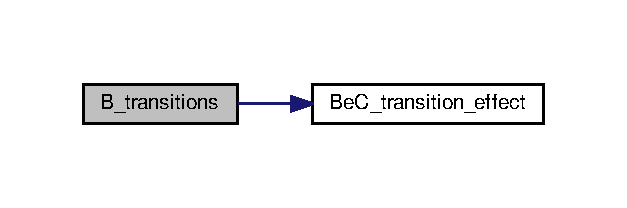
\includegraphics[width=301pt]{statemachine_8c_aa9f36d192c7bb00314ac80a8d2df48a9_cgraph}
\end{center}
\end{figure}


\index{statemachine.\+c@{statemachine.\+c}!Be\+C\+\_\+transition\+\_\+effect@{Be\+C\+\_\+transition\+\_\+effect}}
\index{Be\+C\+\_\+transition\+\_\+effect@{Be\+C\+\_\+transition\+\_\+effect}!statemachine.\+c@{statemachine.\+c}}
\paragraph[{\texorpdfstring{Be\+C\+\_\+transition\+\_\+effect(event\+\_\+t event, void $\ast$data)}{BeC_transition_effect(event_t event, void *data)}}]{\setlength{\rightskip}{0pt plus 5cm}void Be\+C\+\_\+transition\+\_\+effect (
\begin{DoxyParamCaption}
\item[{{\bf event\+\_\+t}}]{event, }
\item[{void $\ast$}]{data}
\end{DoxyParamCaption}
)}\hypertarget{statemachine_8c_a6ee1fe17283b4adb8113f6758ebe126f}{}\label{statemachine_8c_a6ee1fe17283b4adb8113f6758ebe126f}


Definition at line 131 of file statemachine.\+c.



Here is the caller graph for this function\+:\nopagebreak
\begin{figure}[H]
\begin{center}
\leavevmode
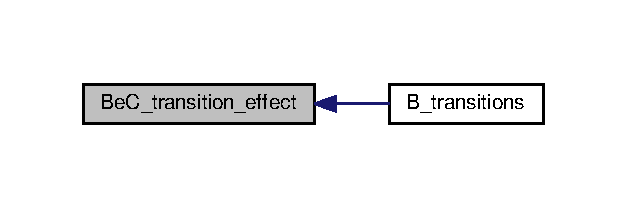
\includegraphics[width=301pt]{statemachine_8c_a6ee1fe17283b4adb8113f6758ebe126f_icgraph}
\end{center}
\end{figure}


\index{statemachine.\+c@{statemachine.\+c}!C\+\_\+entry@{C\+\_\+entry}}
\index{C\+\_\+entry@{C\+\_\+entry}!statemachine.\+c@{statemachine.\+c}}
\paragraph[{\texorpdfstring{C\+\_\+entry(event\+\_\+t event, void $\ast$data)}{C_entry(event_t event, void *data)}}]{\setlength{\rightskip}{0pt plus 5cm}void C\+\_\+entry (
\begin{DoxyParamCaption}
\item[{{\bf event\+\_\+t}}]{event, }
\item[{void $\ast$}]{data}
\end{DoxyParamCaption}
)}\hypertarget{statemachine_8c_ab162221c19b71005e9f3b2d5bed511e2}{}\label{statemachine_8c_ab162221c19b71005e9f3b2d5bed511e2}


State C entry function. 

Every state in a U\+ML state chart can have an optional entry action, which is executed upon entry to a state. Entry actions are associated with states, not transitions. Regardless of how a state is entered, its entry action will be executed.


\begin{DoxyParams}{Parameters}
{\em event} & Triggering event \\
\hline
{\em data} & Data associated with the event \\
\hline
\end{DoxyParams}


Definition at line 193 of file statemachine.\+c.

\index{statemachine.\+c@{statemachine.\+c}!C\+\_\+transitions@{C\+\_\+transitions}}
\index{C\+\_\+transitions@{C\+\_\+transitions}!statemachine.\+c@{statemachine.\+c}}
\paragraph[{\texorpdfstring{C\+\_\+transitions(event\+\_\+t event, void $\ast$data)}{C_transitions(event_t event, void *data)}}]{\setlength{\rightskip}{0pt plus 5cm}const {\bf sm\+\_\+state\+\_\+t}$\ast$ C\+\_\+transitions (
\begin{DoxyParamCaption}
\item[{{\bf event\+\_\+t}}]{event, }
\item[{void $\ast$}]{data}
\end{DoxyParamCaption}
)}\hypertarget{statemachine_8c_a7c2e65f9b16175c058af547044882809}{}\label{statemachine_8c_a7c2e65f9b16175c058af547044882809}


State C transitions function. 

Switching from one state to another is called state transition, and the event that causes it is called the triggering event, or simply the trigger. This function has to be implemented by the state machine designer for each state of the state machine.


\begin{DoxyParams}{Parameters}
{\em event} & Triggering event \\
\hline
{\em data} & Data associated with the event\\
\hline
\end{DoxyParams}
\begin{DoxyReturn}{Returns}
New state in case of external transition. Same state as before in case of self transition. N\+U\+LL in case of internal or no transition. 
\end{DoxyReturn}


Definition at line 211 of file statemachine.\+c.



\subsubsection{Variable Documentation}
\index{statemachine.\+c@{statemachine.\+c}!guard@{guard}}
\index{guard@{guard}!statemachine.\+c@{statemachine.\+c}}
\paragraph[{\texorpdfstring{guard}{guard}}]{\setlength{\rightskip}{0pt plus 5cm}bool guard = false}\hypertarget{statemachine_8c_a7f7d42bd83a62658be38736703dda051}{}\label{statemachine_8c_a7f7d42bd83a62658be38736703dda051}
Guard condition variable as used in U\+ML state chart 

Definition at line 63 of file statemachine.\+c.

\index{statemachine.\+c@{statemachine.\+c}!statemachine\+\_\+state\+\_\+count@{statemachine\+\_\+state\+\_\+count}}
\index{statemachine\+\_\+state\+\_\+count@{statemachine\+\_\+state\+\_\+count}!statemachine.\+c@{statemachine.\+c}}
\paragraph[{\texorpdfstring{statemachine\+\_\+state\+\_\+count}{statemachine_state_count}}]{\setlength{\rightskip}{0pt plus 5cm}const size\+\_\+t statemachine\+\_\+state\+\_\+count = sizeof({\bf statemachine\+\_\+states})/sizeof({\bf statemachine\+\_\+states}\mbox{[}0\mbox{]})}\hypertarget{statemachine_8c_a03b8b76d23b4f034c554518a79c91e7e}{}\label{statemachine_8c_a03b8b76d23b4f034c554518a79c91e7e}
Number of state entries in the state table 

Definition at line 239 of file statemachine.\+c.

\index{statemachine.\+c@{statemachine.\+c}!statemachine\+\_\+states@{statemachine\+\_\+states}}
\index{statemachine\+\_\+states@{statemachine\+\_\+states}!statemachine.\+c@{statemachine.\+c}}
\paragraph[{\texorpdfstring{statemachine\+\_\+states}{statemachine_states}}]{\setlength{\rightskip}{0pt plus 5cm}const {\bf sm\+\_\+state\+\_\+t} statemachine\+\_\+states\mbox{[}$\,$\mbox{]}}\hypertarget{statemachine_8c_aa017019d16cc39ebd231a5f2598d79c0}{}\label{statemachine_8c_aa017019d16cc39ebd231a5f2598d79c0}
{\bfseries Initial value\+:}
\begin{DoxyCode}
= \{
      \{\hyperlink{statemachine_8c_a19575b4361bd5f13002ea2a60abee30e}{A\_entry},      \hyperlink{statemachine_8c_aed25a8dc0c3a7fbe99cb1df00c906308}{A\_transitions},       \hyperlink{statemachine_8c_a6d1d85f00f8d214d50928143924360e8}{A\_exit}\},          
      \{NULL,         \hyperlink{statemachine_8c_aa9f36d192c7bb00314ac80a8d2df48a9}{B\_transitions},       \hyperlink{statemachine_8c_a9268b737532961b741afe6d16b6b27d6}{B\_exit}\},          
      \{\hyperlink{statemachine_8c_ab162221c19b71005e9f3b2d5bed511e2}{C\_entry},      \hyperlink{statemachine_8c_a7c2e65f9b16175c058af547044882809}{C\_transitions},       NULL\}             
\}
\end{DoxyCode}
Statemachine states table 

Definition at line 232 of file statemachine.\+c.


\hypertarget{statemachine_8h}{}\subsection{src/statemachine.h File Reference}
\label{statemachine_8h}\index{src/statemachine.\+h@{src/statemachine.\+h}}


Statemachine for testing purposes -\/ interface.  


{\ttfamily \#include \char`\"{}sm.\+h\char`\"{}}\\*
{\ttfamily \#include \char`\"{}stddef.\+h\char`\"{}}\\*
Include dependency graph for statemachine.\+h\+:\nopagebreak
\begin{figure}[H]
\begin{center}
\leavevmode
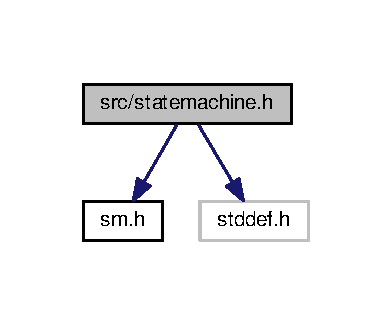
\includegraphics[width=188pt]{statemachine_8h__incl}
\end{center}
\end{figure}
This graph shows which files directly or indirectly include this file\+:\nopagebreak
\begin{figure}[H]
\begin{center}
\leavevmode
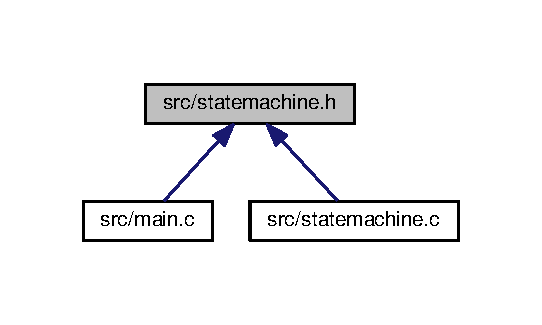
\includegraphics[width=260pt]{statemachine_8h__dep__incl}
\end{center}
\end{figure}
\subsubsection*{Enumerations}
\begin{DoxyCompactItemize}
\item 
enum \hyperlink{statemachine_8h_a91d62a77883891ea8a2ba2209e4736d0}{statemachine\+\_\+event\+\_\+t} \{ \\*
\hyperlink{statemachine_8h_a91d62a77883891ea8a2ba2209e4736d0aa91fb0824da12f8bb3b74dd78fb13b63}{a}, 
\hyperlink{statemachine_8h_a91d62a77883891ea8a2ba2209e4736d0aa06b03e4cd5c7c464c513a95a7fcf9bf}{b}, 
\hyperlink{statemachine_8h_a91d62a77883891ea8a2ba2209e4736d0a776304400122408ea717dde9234fdd2a}{c}, 
\hyperlink{statemachine_8h_a91d62a77883891ea8a2ba2209e4736d0ae8f0ad1953249e38043d318b8f4400d0}{d}, 
\\*
\hyperlink{statemachine_8h_a91d62a77883891ea8a2ba2209e4736d0a5be8d0f77f0d0b6c3724e5c446737d1f}{e}
 \}\begin{DoxyCompactList}\small\item\em Enumeration of events. \end{DoxyCompactList}
\item 
enum \hyperlink{statemachine_8h_aafed9102c6a9aa0ab8753ce5b5cb6f11}{statemachine\+\_\+states\+\_\+t} \{ \hyperlink{statemachine_8h_aafed9102c6a9aa0ab8753ce5b5cb6f11a42a4ade1acd55a49164099104990e09f}{A}, 
\hyperlink{statemachine_8h_aafed9102c6a9aa0ab8753ce5b5cb6f11a3f2a77ecd272aa6d6b5902faa5e5fc68}{B}, 
\hyperlink{statemachine_8h_aafed9102c6a9aa0ab8753ce5b5cb6f11a739ce3f516592d245d16fd8a3893472c}{C}
 \}\begin{DoxyCompactList}\small\item\em Enumeration of states. \end{DoxyCompactList}
\end{DoxyCompactItemize}
\subsubsection*{Variables}
\begin{DoxyCompactItemize}
\item 
const \hyperlink{structsm__state__t}{sm\+\_\+state\+\_\+t} \hyperlink{statemachine_8h_aa017019d16cc39ebd231a5f2598d79c0}{statemachine\+\_\+states} \mbox{[}$\,$\mbox{]}
\item 
const size\+\_\+t \hyperlink{statemachine_8h_a03b8b76d23b4f034c554518a79c91e7e}{statemachine\+\_\+state\+\_\+count}
\end{DoxyCompactItemize}


\subsubsection{Detailed Description}
Statemachine for testing purposes -\/ interface. 

\begin{DoxyCopyright}{Copyright}
Copyright (c) 2013, \href{mailto:marco@bacchi.at}{\tt marco@bacchi.\+at} All rights reserved.
\end{DoxyCopyright}
Redistribution and use in source and binary forms, with or without modification, are permitted provided that the following conditions are met\+:
\begin{DoxyEnumerate}
\item Redistributions of source code must retain the above copyright notice, this list of conditions and the following disclaimer.
\item Redistributions in binary form must reproduce the above copyright notice, this list of conditions and the following disclaimer in the documentation and/or other materials provided with the distribution.
\item The name of the author may not be used to endorse or promote products derived from this software without specific prior written permission.
\end{DoxyEnumerate}

T\+H\+IS S\+O\+F\+T\+W\+A\+RE IS P\+R\+O\+V\+I\+D\+ED BY T\+HE A\+U\+T\+H\+OR ``\+AS IS\textquotesingle{}\textquotesingle{} A\+ND A\+NY E\+X\+P\+R\+E\+SS OR I\+M\+P\+L\+I\+ED W\+A\+R\+R\+A\+N\+T\+I\+ES, I\+N\+C\+L\+U\+D\+I\+NG, B\+UT N\+OT L\+I\+M\+I\+T\+ED TO, T\+HE I\+M\+P\+L\+I\+ED W\+A\+R\+R\+A\+N\+T\+I\+ES OF M\+E\+R\+C\+H\+A\+N\+T\+A\+B\+I\+L\+I\+TY A\+ND F\+I\+T\+N\+E\+SS F\+OR A P\+A\+R\+T\+I\+C\+U\+L\+AR P\+U\+R\+P\+O\+SE A\+RE D\+I\+S\+C\+L\+A\+I\+M\+ED. IN NO E\+V\+E\+NT S\+H\+A\+LL T\+HE A\+U\+T\+H\+OR BE L\+I\+A\+B\+LE F\+OR A\+NY D\+I\+R\+E\+CT, I\+N\+D\+I\+R\+E\+CT, I\+N\+C\+I\+D\+E\+N\+T\+AL, S\+P\+E\+C\+I\+AL, E\+X\+E\+M\+P\+L\+A\+RY, OR C\+O\+N\+S\+E\+Q\+U\+E\+N\+T\+I\+AL D\+A\+M\+A\+G\+ES (I\+N\+C\+L\+U\+D\+I\+NG, B\+UT N\+OT L\+I\+M\+I\+T\+ED TO, P\+R\+O\+C\+U\+R\+E\+M\+E\+NT OF S\+U\+B\+S\+T\+I\+T\+U\+TE G\+O\+O\+DS OR S\+E\+R\+V\+I\+C\+ES; L\+O\+SS OF U\+SE, D\+A\+TA, OR P\+R\+O\+F\+I\+TS; OR B\+U\+S\+I\+N\+E\+SS I\+N\+T\+E\+R\+R\+U\+P\+T\+I\+ON) H\+O\+W\+E\+V\+ER C\+A\+U\+S\+ED A\+ND ON A\+NY T\+H\+E\+O\+RY OF L\+I\+A\+B\+I\+L\+I\+TY, W\+H\+E\+T\+H\+ER IN C\+O\+N\+T\+R\+A\+CT, S\+T\+R\+I\+CT L\+I\+A\+B\+I\+L\+I\+TY, OR T\+O\+RT (I\+N\+C\+L\+U\+D\+I\+NG N\+E\+G\+L\+I\+G\+E\+N\+CE OR O\+T\+H\+E\+R\+W\+I\+SE) A\+R\+I\+S\+I\+NG IN A\+NY W\+AY O\+UT OF T\+HE U\+SE OF T\+H\+IS S\+O\+F\+T\+W\+A\+RE, E\+V\+EN IF A\+D\+V\+I\+S\+ED OF T\+HE P\+O\+S\+S\+I\+B\+I\+L\+I\+TY OF S\+U\+CH D\+A\+M\+A\+GE.

\begin{DoxyVersion}{Version}
0000 
\end{DoxyVersion}
\begin{DoxyAuthor}{Authors}
\href{mailto:marco@bacchi.at}{\tt marco@bacchi.\+at} 
\end{DoxyAuthor}
\begin{DoxyDate}{Date}
2013
\end{DoxyDate}
This statemachine is for testing purposes. It defines three states and some testing transitions between the states. It also makes use of a guard condition and covers exit/entry actions, transition effects and internal transitions.

 
\begin{DoxyImage}
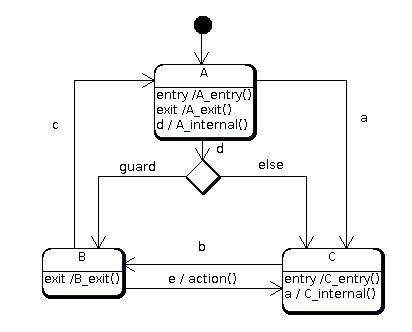
\includegraphics[width=10cm]{sm_test_statemachine.png}
\caption{Statemachine for testing purposes}
\end{DoxyImage}


{\bfseries Changelist}

\tabulinesep=1mm
\begin{longtabu} spread 0pt [c]{*4{|X[-1]}|}
\hline
\rowcolor{\tableheadbgcolor}{\bf Revision}&{\bf Date }&{\bf Name }&{\bf Change  }\\\cline{1-4}
\endfirsthead
\hline
\endfoot
\hline
\rowcolor{\tableheadbgcolor}{\bf Revision}&{\bf Date }&{\bf Name }&{\bf Change  }\\\cline{1-4}
\endhead
0000 &00.\+00.\+00&bacmar&Detailed Change Text \\\cline{1-4}
\end{longtabu}


\subsubsection{Enumeration Type Documentation}
\index{statemachine.\+h@{statemachine.\+h}!statemachine\+\_\+event\+\_\+t@{statemachine\+\_\+event\+\_\+t}}
\index{statemachine\+\_\+event\+\_\+t@{statemachine\+\_\+event\+\_\+t}!statemachine.\+h@{statemachine.\+h}}
\paragraph[{\texorpdfstring{statemachine\+\_\+event\+\_\+t}{statemachine_event_t}}]{\setlength{\rightskip}{0pt plus 5cm}enum {\bf statemachine\+\_\+event\+\_\+t}}\hypertarget{statemachine_8h_a91d62a77883891ea8a2ba2209e4736d0}{}\label{statemachine_8h_a91d62a77883891ea8a2ba2209e4736d0}


Enumeration of events. 

\begin{Desc}
\item[Enumerator]\par
\begin{description}
\index{a@{a}!statemachine.\+h@{statemachine.\+h}}\index{statemachine.\+h@{statemachine.\+h}!a@{a}}\item[{\em 
a\hypertarget{statemachine_8h_a91d62a77883891ea8a2ba2209e4736d0aa91fb0824da12f8bb3b74dd78fb13b63}{}\label{statemachine_8h_a91d62a77883891ea8a2ba2209e4736d0aa91fb0824da12f8bb3b74dd78fb13b63}
}]Special event used for transiting from state A to state C \index{b@{b}!statemachine.\+h@{statemachine.\+h}}\index{statemachine.\+h@{statemachine.\+h}!b@{b}}\item[{\em 
b\hypertarget{statemachine_8h_a91d62a77883891ea8a2ba2209e4736d0aa06b03e4cd5c7c464c513a95a7fcf9bf}{}\label{statemachine_8h_a91d62a77883891ea8a2ba2209e4736d0aa06b03e4cd5c7c464c513a95a7fcf9bf}
}]Same as event a, but this time for transition from state C to state B \index{c@{c}!statemachine.\+h@{statemachine.\+h}}\index{statemachine.\+h@{statemachine.\+h}!c@{c}}\item[{\em 
c\hypertarget{statemachine_8h_a91d62a77883891ea8a2ba2209e4736d0a776304400122408ea717dde9234fdd2a}{}\label{statemachine_8h_a91d62a77883891ea8a2ba2209e4736d0a776304400122408ea717dde9234fdd2a}
}]Event used for transition from state B to A \index{d@{d}!statemachine.\+h@{statemachine.\+h}}\index{statemachine.\+h@{statemachine.\+h}!d@{d}}\item[{\em 
d\hypertarget{statemachine_8h_a91d62a77883891ea8a2ba2209e4736d0ae8f0ad1953249e38043d318b8f4400d0}{}\label{statemachine_8h_a91d62a77883891ea8a2ba2209e4736d0ae8f0ad1953249e38043d318b8f4400d0}
}]Event used to demonstrate a trnsition with an external guard condition \index{e@{e}!statemachine.\+h@{statemachine.\+h}}\index{statemachine.\+h@{statemachine.\+h}!e@{e}}\item[{\em 
e\hypertarget{statemachine_8h_a91d62a77883891ea8a2ba2209e4736d0a5be8d0f77f0d0b6c3724e5c446737d1f}{}\label{statemachine_8h_a91d62a77883891ea8a2ba2209e4736d0a5be8d0f77f0d0b6c3724e5c446737d1f}
}]Event used to demonstrate an extrnal transition with a transition effect \end{description}
\end{Desc}


Definition at line 61 of file statemachine.\+h.

\index{statemachine.\+h@{statemachine.\+h}!statemachine\+\_\+states\+\_\+t@{statemachine\+\_\+states\+\_\+t}}
\index{statemachine\+\_\+states\+\_\+t@{statemachine\+\_\+states\+\_\+t}!statemachine.\+h@{statemachine.\+h}}
\paragraph[{\texorpdfstring{statemachine\+\_\+states\+\_\+t}{statemachine_states_t}}]{\setlength{\rightskip}{0pt plus 5cm}enum {\bf statemachine\+\_\+states\+\_\+t}}\hypertarget{statemachine_8h_aafed9102c6a9aa0ab8753ce5b5cb6f11}{}\label{statemachine_8h_aafed9102c6a9aa0ab8753ce5b5cb6f11}


Enumeration of states. 

Enumeration of states of the state machine. This enumeration has to match with the entries in the state table! \begin{Desc}
\item[Enumerator]\par
\begin{description}
\index{A@{A}!statemachine.\+h@{statemachine.\+h}}\index{statemachine.\+h@{statemachine.\+h}!A@{A}}\item[{\em 
A\hypertarget{statemachine_8h_aafed9102c6a9aa0ab8753ce5b5cb6f11a42a4ade1acd55a49164099104990e09f}{}\label{statemachine_8h_aafed9102c6a9aa0ab8753ce5b5cb6f11a42a4ade1acd55a49164099104990e09f}
}]State with entry/exit action, an internal transition, and external transition and an external contition with guard condition \index{B@{B}!statemachine.\+h@{statemachine.\+h}}\index{statemachine.\+h@{statemachine.\+h}!B@{B}}\item[{\em 
B\hypertarget{statemachine_8h_aafed9102c6a9aa0ab8753ce5b5cb6f11a3f2a77ecd272aa6d6b5902faa5e5fc68}{}\label{statemachine_8h_aafed9102c6a9aa0ab8753ce5b5cb6f11a3f2a77ecd272aa6d6b5902faa5e5fc68}
}]State with exit action, an external tranistion and another external transition with a transition effect \index{C@{C}!statemachine.\+h@{statemachine.\+h}}\index{statemachine.\+h@{statemachine.\+h}!C@{C}}\item[{\em 
C\hypertarget{statemachine_8h_aafed9102c6a9aa0ab8753ce5b5cb6f11a739ce3f516592d245d16fd8a3893472c}{}\label{statemachine_8h_aafed9102c6a9aa0ab8753ce5b5cb6f11a739ce3f516592d245d16fd8a3893472c}
}]State with entry action, internal tranition and eternal transition \end{description}
\end{Desc}


Definition at line 74 of file statemachine.\+h.



\subsubsection{Variable Documentation}
\index{statemachine.\+h@{statemachine.\+h}!statemachine\+\_\+state\+\_\+count@{statemachine\+\_\+state\+\_\+count}}
\index{statemachine\+\_\+state\+\_\+count@{statemachine\+\_\+state\+\_\+count}!statemachine.\+h@{statemachine.\+h}}
\paragraph[{\texorpdfstring{statemachine\+\_\+state\+\_\+count}{statemachine_state_count}}]{\setlength{\rightskip}{0pt plus 5cm}const size\+\_\+t statemachine\+\_\+state\+\_\+count}\hypertarget{statemachine_8h_a03b8b76d23b4f034c554518a79c91e7e}{}\label{statemachine_8h_a03b8b76d23b4f034c554518a79c91e7e}
Number of state entries in the state table 

Definition at line 239 of file statemachine.\+c.

\index{statemachine.\+h@{statemachine.\+h}!statemachine\+\_\+states@{statemachine\+\_\+states}}
\index{statemachine\+\_\+states@{statemachine\+\_\+states}!statemachine.\+h@{statemachine.\+h}}
\paragraph[{\texorpdfstring{statemachine\+\_\+states}{statemachine_states}}]{\setlength{\rightskip}{0pt plus 5cm}const {\bf sm\+\_\+state\+\_\+t} statemachine\+\_\+states\mbox{[}$\,$\mbox{]}}\hypertarget{statemachine_8h_aa017019d16cc39ebd231a5f2598d79c0}{}\label{statemachine_8h_aa017019d16cc39ebd231a5f2598d79c0}
Statemachine states table 

Definition at line 232 of file statemachine.\+c.


%--- End generated contents ---

% Index
\newpage
\phantomsection
\clearemptydoublepage
\addcontentsline{toc}{section}{Index}
\printindex

\end{document}
